\documentclass[conference]{IEEEtran}

\usepackage[inline]{enumitem}
\usepackage[bookmarks]{hyperref}
\usepackage[inline]{enumitem}
\usepackage{algorithm}
\usepackage{algpseudocode}
\usepackage[dvipsnames]{xcolor}
\usepackage{pgfplots,pgfplotstable}
\usepackage{array}
\usepackage{subcaption}

\graphicspath{{images/}}
\DeclareGraphicsExtensions{.pdf,.jpeg,.png,.eps}

% correct bad hyphenation here
\hyphenation{op-tical net-works semi-conduc-tor}

\def\checkmark{\tikz\fill[scale=0.4] (0,.35) -- (.25,0) -- (1,.7) -- (.25,.15) -- cycle;}
\newcommand*\circled[1]{\raisebox{.5pt}{\textcircled{\raisebox{-.9pt} {#1}}}}

\definecolor{LighterGray}{RGB}{232, 232, 232}
\definecolor{LightGray}{RGB}{194, 194, 194}
\definecolor{Gray}{RGB}{150, 150, 150}
\definecolor{DarkGray}{RGB}{102, 102, 102}
\definecolor{DarkerGray}{RGB}{56, 56, 56}

\pgfplotstableread{evaluation_results/overall_time.dat}{\LoadOverallTime}
\pgfplotstableread{evaluation_results/overall_write.dat}{\LoadOverallWrite}
% \pgfplotstableread{evaluation_results/lru_time.dat}{\LoadLRUTime}
% \pgfplotstableread{evaluation_results/lru_write.dat}{\LoadLRUWrite}
\pgfplotstableread{evaluation_results/data_modifies_between_checkpointing.dat}{\LoadModifies}
\pgfplotstableread{evaluation_results/cache_miss_latency.dat}{\LoadLatency}
\pgfplotstableread{evaluation_results/overall_time_different_pool_size.dat}{\LoadOverallTimeDifferentPoolSize}
\pgfplotstableread{evaluation_results/overall_write_different_pool_size.dat}{\LoadOverallWriteDifferentPoolSize}
% \pgfplotstableread{evaluation_results/wd4_every_checkpointing_period_length.original}{\LoadWDFourEveryCheckpointingPeriodLength}
\pgfplotstableread{evaluation_results/wd4_checkpointing_pages_between_checkpointing.dat}{\LoadWDFourCheckpointingPagesBetweenCheckpointing}
\pgfplotstableread{evaluation_results/wd4_pool_full_timing.original}{\LoadWDFourPoolFullTiming}
\pgfplotstableread{evaluation_results/wd4_finished_requests_between_checkpointing.original}{\LoadWDFourFinishedRequestsPerCheckpointing}
\pgfplotstableread{evaluation_results/wd5_checkpointing_pages_between_checkpointing.dat}{\LoadWDFiveCheckpointingPagesBetweenCheckpointing}
\pgfplotstableread{evaluation_results/wd5_pool_full_timing.original}{\LoadWDFivePoolFullTiming}
% \pgfplotstableread{evaluation_results/overall_time_metadata.dat}{\LoadOverallTimeMetadata}
% \pgfplotstableread{evaluation_results/overall_time_metadata2.dat}{\LoadOverallTimeMetadataTwo}

\pgfplotsset{select row/.style={x filter/.code={\ifnum\coordindex=#1\else\def\pgfmathresult{}\fi}}}

\begin{document}

\title{Optimizing Memory-based Checkpointing in Hybrid-Memory System}


\author{\IEEEauthorblockN{Michael Shell}
\IEEEauthorblockA{School of Electrical and\\Computer Engineering\\
Georgia Institute of Technology\\
Atlanta, Georgia 30332--0250\\
Email: http://www.michaelshell.org/contact.html}
\and
\IEEEauthorblockN{Homer Simpson}
\IEEEauthorblockA{Twentieth Century Fox\\
Springfield, USA\\
Email: homer@thesimpsons.com}
\and
\IEEEauthorblockN{James Kirk\\ and Montgomery Scott}
\IEEEauthorblockA{Starfleet Academy\\
San Francisco, California 96678--2391\\
Telephone: (800) 555--1212\\
Fax: (888) 555--1212}}

% make the title area
\maketitle


\begin{abstract}
    Fault tolerance is a crucial problem for exascale systems.
    Checkpointing is common used to address this problem, however, in HDD-based high performance computing systems, it incurs huge overhead as its frequency increases.
    Memory-based checkpointing mitigates such huge overhead by sharing data between working memory and checkpoint, but encounters a new problem that any modification on working memory will corrupt the consistency of checkpoint.
    Traditional memory-based checkpointing adopts logging or copy-on-write to resolve this problem, with inevitable extra writes.
    For next generation memory system, which is composed by DRAM and emerging non-volatile memory, such as phase change memory (PCM), extra writes could be severe because the low PCM writing performance.
    Existing research has leveraged PCM to perform checkpointing, but they still suffer from unexpected double-space or double-writes because they treat PCM as storage device instead of memory.

    In this paper, we propose a memory-based checkpointing mechanism for next generation memory system, namely hybrid memory system.
    By utilizing our checkpointing-dedicated fine-grained address remapping mechanism, called Twins Page Mapping, we could keep checkpoint consistent without many extra writes.
    Twins Page Mapping maps one physical page to two PCM pages, called Base Page and Derivation Page respectively.
    To reduce extra writes, these pages are split into cache lines.
    If the $n_{th}$ cache line of the Base Page stores a portion of checkpoint, further modification on it will be redirected to the $n_{th}$ cache line of the Derivation page, and vice-versa.
    Such design reduces the metadata in that every cache line has only two possible addresses, thus every cache line needs only one bit metadata to indicate which address stores checkpoint.
    Our evaluation covers various workloads, and demonstrates at most 5.99x writes reduction and at most 1.88x speedup.
\end{abstract}

\IEEEpeerreviewmaketitle{}

\section{Introduction}

% 1 page

With fast evolution of today's scientific research, future researchers require exascale systems to perform their scientific simulations.
One of the most serious problems in exascale computing is the reliability issue.
Specifically, the mean time between failures (MTBF) will become very short in the exascale systems because of extremely large number of cores to use in parallel.
The replica execution mechanism~\cite{detection-sc12,Benson-SED,cite:scalable-rep,cite:scal-rep2} is unqualified for the exascale fault tolerance, because it needs to launch extra processes/ranks to process the same work as the original processes, such that the total number of cores/process will double or triple.
By contrast, checkpoint/restart mechanism protects the execution by saving the runtime memory periodically, avoiding the waste of the resources.
Checkpoint overhead, however, could be too huge to neglect.
Specifically, high frequency checkpointing may cause over 50\% performance degradation~\cite{stearley_rmpi_2011} or nearly 80\% of the total I/O traffic~\cite{petrini_scaling_2002} in traditional HDD-based High Performance Computing (HPC) systems.

Memory-based Checkpointing (storing checkpoints in memory instead of hard disks) has been proposed~\cite{sorin_safetynet_2002, prvulovic_revive_2002} for years, in order to address the huge checkpoint overhead issue.
The advantage of memory-based checkpointing method is not only the low access latency and byte-addressability supplied by DRAM, but little data copy time to be incurred because the working memory just needs to be marked as checkpointing memory upon the checkpointing request.

To mitigate the volatile issue of DRAM, non-volatile memory (NVM), such as phase-change memory (PCM), has gained a lot of attention for next-generation memory system, since NVM can achieve a comparable reading performance as DRAM\@.
Its high writing latency and limited retainability, however, still impede the performance significantly.
As such, hybrid memory system with both DRAM and PCM is proposed to overcome these drawbacks.

In a hybrid memory system, extra writes could be a very severe problem because of the low PCM writing performance and the logging design or copy-on-write operations.
Memory-based checkpointing shares data between working memory and checkpointing memory, such that any modification on working memory will corrupt its consistency with the checkpointing memory.
To this end, traditional memory-based checkpointing adopts logging or copy-on-write to reserve checkpointing memory, introducing extra writes inevitably.
In particular, logging incurs 1x extra writes because it needs to write both new and old data, and copy-on-write incurs variable extra writes as it has to write a whole page even partial data is unmodified.
Although existing research~\cite{dong_leveraging_2009, kannan_optimizing_2013, gao_real-time_2015} has leveraged PCM to perform the checkpointing, they still suffer from unexpected double-space or double-writes because they treat the PCM as storage device instead of memory (storage-based checkpointing cannot share data between working memory and checkpointing memory).

In this paper, we propose a novel memory-based checkpointing mechanism, wherein the checkpointing overhead can be minimized by leveraging the features of hybrid memory system.
The key contributions are listed as follows:

\begin{enumerate}
    \item We propose a checkpointing-dedicated fine-grained address remapping mechanism, namely \emph{Twins Page Mapping}, to resolve the checkpointing consistency issue, with much less overhead than logging and copy-on-write.
        Twins Page Mapping is able to identify the address of working memory and checkpoint, and translate memory request to the address of working memory in the granularity of cache line.
        Specifically, Twins Page Mapping maps one physical page to two PCM pages, called Base Page and Derivation Page respectively.
        To reduce extra writes, these pages are split into cache lines.
        If the $n_{th}$ cache line of the Base Page stores a portion of checkpointing memory, further modification on it will be redirected to the $n_{th}$ cache line of the Derivation page, and vice-versa.
        Such a design can effectively avoid corrupting checkpoint, and also reduce the metadata in that every cache line has only two possible addresses.
        That is, every cache line needs only one bit metadata to indicate which address stores the checkpointing memory.
    \item Coordinating with hybrid memory system, we also propose two optimization strategies that could reduce address translation count and the size of metadata stored in memory controller respectively.
        Besides that, a hardware-based Derivation Page management mechanism is proposed to improve efficiency and constrain the storage overhead.
    \item We implement our checkpointing system with common used simulation tools and evaluate its performance under various workloads.
        The evaluation demonstrates at most 5.99x writes reduction and at most 1.88x speedup.
\end{enumerate}

The rest of this paper is organized as follows.
Section~\ref{sec:motivation} elaborates the motivation of our work.
Section~\ref{sec:design} describes the design of our checkpointing system and key mechanism.
Section~\ref{sec:implementation} introduces implementation details.
Section~\ref{sec:evaluation} presents the evaluation and results, followed by a conclusion in Section~\ref{sec:conclusion}.

\section{Background and Design Motivation}\label{sec:motivation}
% 3 pages

In this section, we analyze the pros and cons of the traditional memory-based checkpointing technology and PCM-based checkpointing technology.

% In this section, we first introduce hybrid memory system, which is a promising trend for future HPC system.
% Then we elaborate the problems of porting traditional memory-based checkpointing and state-of-the-art PCM-assisted checkpointing technologies into hybrid memory system respectively.

% \subsection{PCM and Hybrid-Memory System}
%
% After decades of development, NVM technologies becomes a promising candidate of DRAM\@.
% Among different kinds of NVM, PCM is the one which is expected to be a useful medium in near future~\cite{condit_better_2009}.
% As a memory technology, PCM can connect to memory bus to gain memory specific advantages such as high performance access, byte-addressability, low-level parallelism etc.
% But compared with existing commercial SRAM and DRAM technologies, PCM has relative bad performance.
% Read from PCM is several times slower than DRAM\@.
% Also compared with DRAM, one magnitude larger write latency, limited retainability, high active energy consuming results expensive PCM write.
% These shortages make it still can not replace DRAM\@.
%
% To gain the high performance advantage from DRAM and the large capacity and non-volatile features from PCM, Hybrid-Memory System is proposed.
% Two typical architectures are:
% \begin{enumerate*}
% \item DRAM acts as the cache of PCM,
% \item DRAM and PCM share address space.
% \end{enumerate*}
% Using DRAM as the cache of PCM can mitigate the performance degradation caused by PCM's relative low performance, and latest work such as~\cite{qureshi_scalable_2009, qureshi_morphable_2010, park_power_2011, yoon_row_2012, ham_disintegrated_2013, zhou_leveraging_2013} chooses this architecture as their target system, too.
% This architecture seems more promising so this paper focuses on it.
% In this architecture, all memory access requests are checked whether it hits DRAM cache first.
% If hits, DRAM will service theses requests.
% Otherwise, the request page will be read from PCM\@.

% Researchers have done a lot of work on hybrid-memory system from different aspects.
% \cite{qureshi_scalable_2009, dhiman_pdram_2009, ramos_page_2011} propose different architecture to improve system performance.
% \cite{wu_car_2012} focuses on the security of PCM and designs address remapping to defend intended attack.
% \cite{park_power_2011, ham_disintegrated_2013} exploits the low standby power of PCM to build an energy saving system.
% Hybrid-memory system becomes a promising trend.

%\subsection{Memory-based Checkpointing}\label{sec:motivation-in_memory_checkpointing}

% In hybrid memory system, although PCM is non-volatile, CPU context information and partial working memory is stored in volatile memories.
% Hence fault-tolerance mechanism is still necessary for hybrid memory system.
% Since PCM acts as memory, and it has the advantages of large capacity and non-volatile, memory-based checkpointing could be a promising fault tolerance solution.

% Memory-based checkpointing~\cite{sorin_safetynet_2002, prvulovic_revive_2002} stores checkpoint in memory and benefits from two aspects.
% First, data access is quite fast for the sake of memory system's high performance.
% Second, during checkpointing, it just marks working memory as checkpoint without data copy.
% So memory-based checkpointing is quite lightweight.
% However, while it is efficient, it encounters two new problems, namely persistent data store and checkpoint consistency.

% Researchers have proposed several memory-based checkpointing systems for DRAM-based memory~\cite{sorin_safetynet_2002, prvulovic_revive_2002}.

% \begin{figure}
%     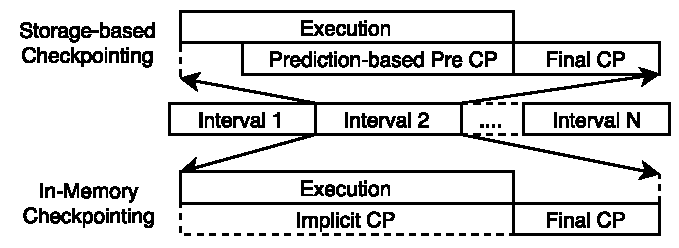
\includegraphics[width=\columnwidth]{storage_and_memory}
%     \caption{Timing diagrams of Storage-based Checkpointing and memory-based Checkpointing. The execution of application is split to multiple intervals. In each interval, application will execute for a while and generate a checkpoint at the end of the interval.[obsolete]}
% \label{fig:storage_and_memory}
% \end{figure}

% As shown in the Figure~\ref{fig:storage_and_memory},

% Memory-based checkpointing shrinks system downtime by implicit checkpointing, which means implying checkpointing to application execution.
% The most time-consuming part of checkpointing is the procedure of copying application data to checkpoint storage.
% But because memory-based checkpointing chooses memory as checkpoint storage, the procedure of application writing data to memory during execution is the same as the procedure of copying application data to checkpoint storage.

% Memory-based checkpointing relieves the heavy data copy by implicit checkpointing, but it encounters two new problems, namely persistent data store and checkpoint consistency.

Memory-based checkpointing \cite{} effectively mitigates the heavy data copying issue during checkpointing, while it suffers from the volatile issue of DRAM. 
Although this issue can be resolved by adopting NVM in a hybrid memory system, checkpointing consistency problem will be further introduced in turn, as shown in Figure~\ref{fig:consistency}. Such a problem will be rather more critical because NVM works very inefficiently on the extra writes incurred.

% Persistent data store problem is critical in DRAM-base memory system because DRAM is volatile.
% Checkpoint data stored in DRAM will lose when node failure happens.
% To build a logical non-volatile DRAM, prior work\cite{prvulovic_revive_2002} proposes to make data redundant across nodes.
% However, it incurs overhead to maintain this redundant policy.
% In hybrid-memory system, memory contains non-volatile medium, so the persistent data store problem is naturally resolved as we place checkpoint to PCM\@.
% The data redundancy policy used in traditional memory-based checkpointing system becomes a redundancy.

Memory-based checkpointing marks working memory as checkpointing memory instead of copying them to the checkpoint storage.
Thus, after setting a checkpoint, there will be only one copy of data in memory, which has two roles - working memory and checkpointing memory, meanwhile.
Later modifications on working memory will corrupt checkpointing memory and leave it to inconsistent state, such that the checkpointing data is no longer available to use.

% After checkpointing, these data constructs a checkpoint and can be used to recover to previous state.
% Then a write request comes and try to overwrite data B with data X.
% If we do nothing for this write request, what left in memory is data A, data X and data C to H, which is not a valid checkpoint and can not be used to recover.

\begin{figure}
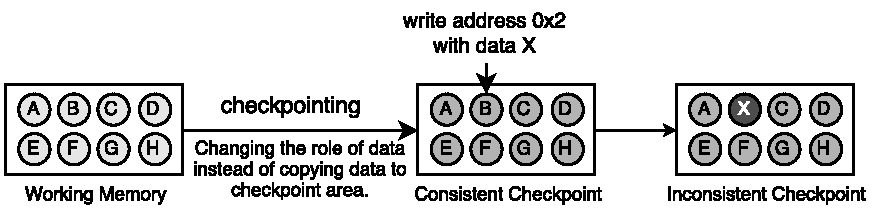
\includegraphics[width=\columnwidth]{consistency-2}
\caption{Consistency Problem of Memory-based Checkpointing.
Memory-based Checkpointing only changes the role of working memory to checkpoint without copy.
Thus checkpoint and working memory share the same data.
The modification of working memory also means the modification of checkpoint.
Such modification corrupts the consistency of checkpoint and makes it can not be used for recovery.
}
\label{fig:consistency}
\end{figure}

Existing solutions that deal with the checkpointing consistency issue include logging mechanism and copy-on-write.

Logging mechanism has two modes, \emph{redo logging} and \emph{undo logging}, which suffer from the same problems, so we explain it by using only undo logging mode without loss of generality.
The undo logging mechanism copies old data to a logging area before storing them, which may incur extra writing cost because of the two steps involved: the first step is copying old data to logging area (one write) and the second step writes new data to original address (one more write).
Note that every logging entry also requires to write metadata (such as data address), so the undo logging mechanism actually incurs over 1x extra writes when it needs to save data.

Copy-on-Write is an address remapping mechanism, which modifies page table entry and maps the linear address of old area to a newly allocated area.
The new area is generally a 4KB or 4MB page, and copy-on-write has to write the whole page even if only a few of data are actually changed in the page.
% The write of these unmodified data is extra.
We conducted an experiment to characterize the extra writes that copy-on-write may incur, with the size of cache line (more detailed experimental setting is described in Section \ref{sec:evaluation_methodology}). The extra writes are measured using the number of unmodified cache lines between two consecutive checkpoints.
Figure~\ref{fig:modifies} clearly confirms that Page level copy-on-write may incur massive extra writes. Specifically, the average extra write ratio is up to 51.3\%, and there are even four applications whose extra write ratios are greater than 90\%.
There are only 5 applications (from among a total of 28 applications) with 10\% extra write ratios. Obviously, reducing the granularity of copy-on-write from page to cache line will reduce extra writes. However, a general-purpose fine-grained copy-on-write may cause unacceptable memory management overheads, which make it unfeasible in turn. As such, a new technology is required to resolve checkpoint consistency with less writes. %sdi: as for the statement "unacceptable memory management overheads": really? any evidence such as references to put here? s

\begin{figure}
    \begin{tikzpicture}
        \begin{axis}[
                ybar,
                bar width=4pt,
                height=4cm,
                ymin=0,
                xtick=data,
                xticklabels from table={\LoadModifies}{program},
                xticklabel style={rotate=45, font=\tiny, anchor=north east},
                ylabel=Extra Write,
                ylabel style={font=\small},
                yticklabel=\pgfmathprintnumber{\tick}\,\%,
                extra y ticks={10, 90},
                extra y tick labels={$10\%$, $90\%$},
                % extra y tick style={grid=major, densely dashed, very thin, gray, font=\footnotesize, yticklabel={$51\%$}},
                extra y tick style={grid=major, densely dashed, font=\scriptsize},
                enlarge x limits=0.04,
                bar shift=0pt,
                %enlarge y limits={upper, value=0.2},
                %nodes near coords,
                %every node near coord/.append style={rotate=90, anchor=west, font=\small},
                width=\columnwidth,
            ]
            \draw[DarkGray, very thin, densely dashed] (axis cs:\pgfkeysvalueof{/pgfplots/xmin},50) -- (axis cs:\pgfkeysvalueof{/pgfplots/xmax},50);
            \addplot[color=DarkGray, fill=gray] table[x expr=\coordindex, y=modifies] \LoadModifies;
            \addplot[color=DarkGray, fill=LightGray] table[x expr=\coordindex, y=modifies, select row=28] \LoadModifies;
            \node[pin = {[font=\tiny, color=DarkGray, pin distance=7pt] above:51.3\%}] at (axis cs:28, 50) {};
        \end{axis}
    \end{tikzpicture}
    \caption{The Percentage of Extra Writes of Page Level Copy-on-Write}
    % \caption{Extra Writes of Page Level Copy-on-Write compared with Cache line Level Copy-on-Write}
    % \caption{The Count of Modified Cache Lines in a Page between Two Checkpointings}
\label{fig:modifies}
\end{figure}

%To summarize, logging and copy-on-write incur lots of extra writes.
%In traditional DRAM-based memory system, these extra writes have limited influence because of the high performance of DRAM\@.
%However, extra writes could be critical when we port such mechanisms to hybrid memory system, which has a medium with relative bad write performance.
% However, porting such mechanisms to hybrid memory system could potentially slow down system
% In contrast, extras writes on PCM become critical because of PCM's relative bad write performance.
%Thus, we need a new strategy to overcome checkpoint consistency problem with less writes.
% The extra writes slow down system and cut down the service life of PCM (see Section~\ref{sec:evaluation_overall}).

% Furthermore, the bad write performance of PCM enlarges the overhead of final checkpointing phase.
% Final checkpointing suspends application and copies all data stored over checkpoint storage level to checkpoint storage.
% memory-based checkpointing in DRAM-based main memory system copies the data from CPU cache to logical non-volatile DRAM, while hybrid-memory system needs to copy data from DRAM to PCM\@.
% Final checkpointing is lightweight and quick because CPU cache is just multiple megabytes and DRAM's low write latency.
% But in hybrid-memory system, DRAM capacity is gigabytes and PCM write is relative slow.
% These two factors lead to a long final checkpointing phase.

%\subsection{The Problems in PCM-assisted Checkpointing}

In addition to the above-mentioned memory-based checkpointing mechanism with potential checkpointing consistency issue, many researchers~\cite{dong_leveraging_2009, kannan_optimizing_2013, gao_real-time_2015} utilize PCM as the checkpointing device, in order to reach a tradeoff between the higher checkpointing performance and checkpointing consistency.
Although the system can access PCM directly through memory bus and PCM supplies byte-addressability, the memory used by applications cannot be dynamically allocated from PCM, such that PCM can only serve as a storage device from the perspective of operating system.
This is why most existing PCM-based checkpointing mechanisms actually adopt the traditional storage-based checkpointing methods instead.

Unlike memory-based checkpointing, storage-based checkpointing does not share working memory and checkpointing memory, because of the volatile issue of traditional DRAM.
As for a hybrid memory system, however, such a storage-based checkpointing design cannot make full use of the non-volatile feature of memory. What is even worse is that the isolation of working memory and checkpointing memory may result in an instant double size of the working memory, in that a checkpoint generated during the execution is actually a snapshot of the working memory. This will definitely introduce a very huge burden on the memory capacity especially for the next-generation exascale applications with extremely large volume of data to process.
On the other hand, redundant data incurs redundant writing cost, especially for the hybrid memory system because PCM suffers from poor data writing performance. Therefore, it is necessary to tailor a new checkpointing solution for the hybrid memory system, in order to maximize its checkpointing performance. 

% Mona is one of these state-of-the-art PCM-assisted checkpointing systems.
% Mona splits checkpointing to partial checkpointing phase and final checkpointing phase, and focuses on the optimization of partial checkpointing.
% It also exploits the advantages of place PCM on memory bus and introduces rank-level load balancing.

% However, prior works such as Mona treat PCM as storage instead of memory.
% Although they propose to use PCM as memory, but they aim to memory's physical characteristics.
% By connecting to memory bus, system can use the byte-address ability of PCM\@.
% And memory access requires no context switch so that the performance will be higher than accessing device.
% But since the operating system on prior works does not allocate memory in PCM, PCM is storage logically.

% Using PCM as storage instead of memory has performance degradation caused by swapping.

% \begin{enumerate}

% Big data applications require more and more memory.
% If we use PCM as storage, the memory capacity is determined by DRAM\@.
% Because of the low density of DRAM, building a large DRAM-based memory is not as feasible as using PCM\@.
% Insufficient memory will make operating system activating swapping technology to meet the memory demand of big data applications.
%
% Swapping will cause three problems.
% \begin{enumerate*}
% 	\item Performance degradation caused by data copying.
% 	Swapping copies pages from memory to swap space if system can not find a free page to allocate or the pages have not been accessed for a long time.
% 	Even if we place swap space in PCM, swapping still incurs overhead and is slower than access memory directly.
% 	\item Data redundancy.
% 	As we place both swap space and checkpoint data in PCM, the data in swap space will be redundant with checkpoint data.
% 	\item Redundant data copying during checkpointing process.
% 	Checkpointing can not recognize whether the data is stored in DRAM or swap space, so it may try to copy data stored in swap space to PCM\@.
% 	Read the data stored in swap space makes system reads these data from PCM to swap them into memory, and they were written back to the checkpoint storage area in PCM again by checkpointing process.
% 	Reads and writes in this process are all redundant.
% \end{enumerate*}

% Besides the performance degradation caused by using PCM as storage, prediction-based pre checkpointing in storage-based checkpointing causes redundant writes.
% Prediction-based Pre Checkpointing is a technology for paralleling checkpointing and application execution, as illustrated in Figure~\ref{fig:storage_and_memory}.
% Workloads have some idle periods generally.
% For CPU-intensive workloads running in hybrid-memory system, PCM is idle for 60\%$\sim$90\% of time as we evaluate.
% Memory-intensive workloads also have thousands of nanoseconds idle period\cite{huang_improving_2005}.
% So to make full use of these idle periods and reduce application suspend time caused by final checkpointing, pre checkpointing utilizes these idle periods to perform checkpointing.
% The performance of pre checkpointing relies on two prediction, which are cold data prediction and idle period distribution prediction.
% Apparently, perdition algorithms will not achieve 100\% precision.
% Prediction deviation incurs redundant writes, and just as Mona evaluates, it has 28\% redundant writes.

\section{System Design}\label{sec:design}

This section presents the overview of our checkpointing system first.
Then we introduce Twins Page Mapping, which is able to resolve the checkpoint consistency problem with low overhead.
% , followed by two key optimization of it.

\subsection{Overview}

The goal of our checkpointing is to tolerate failures of hybrid memory system efficiently.
We focus on the optimization of checkpointing, and adopt common methods for failure detection and recovery (cite).
Theoretically, our checkpointing system can handle different failure models if it collaborates with appropriate failure detection technology.
Hence we suppose a fail-stop model in this paper for the sake of simplicity.

Hybrid memory system has two typical architectures:
\begin{enumerate*}
\item DRAM acts as the cache of PCM,
\item DRAM and PCM share address space.
\end{enumerate*}
Using DRAM as the cache of PCM can mitigate the performance degradation caused by PCM's relative low performance, and latest work such as~\cite{qureshi_scalable_2009, qureshi_morphable_2010, park_power_2011, yoon_row_2012, ham_disintegrated_2013, zhou_leveraging_2013} chooses this architecture as their target system, too.
This architecture seems more promising so this paper focuses on it.
In this architecture, all memory access requests are checked whether it hits DRAM cache first.
If hits, DRAM will service theses requests.
Otherwise, the request page will be read from PCM\@.

% \begin{figure*}[t!]
%     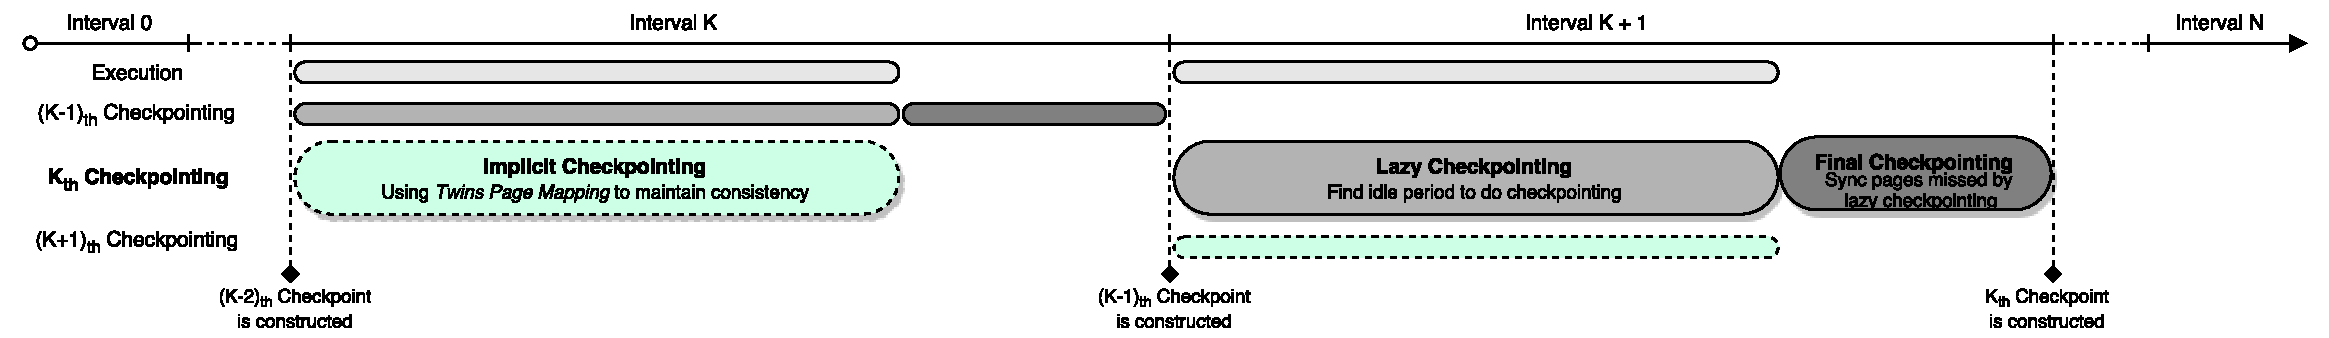
\includegraphics[width=\textwidth]{overview-lazy-2}
%     \caption{Overview of XXX Checkpointing}
% \label{fig:overview}
% \end{figure*}

% \begin{figure}[t!]
%     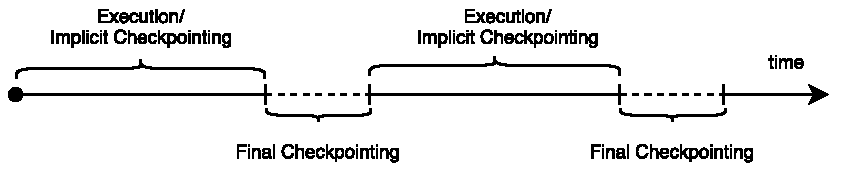
\includegraphics[width=\columnwidth]{overview_simple}
%     \caption{Overview of XXX Checkpointing}
% \label{fig:overview}
% \end{figure}

We split the application execution into multiple intervals.
Each interval is composed by two periods.
One is application execution period, and the other is checkpointing period.
At the end of each interval, a checkpoint is generated.

% To address checkpoint consistency problem during this period, we propose Twins Page Mapping.
% In this period, cache eviction is responsible for
% Cache eviction during execution period implies checkpointing, because checkpointing process is copying modified working memory to PCM\@.
% We call this process \textit{Implicit Checkpointing}.
%
% Checkpointing needs to copy modified working memory to PCM, so cache eviction during execution period also implies checkpointing.

% Execution period resumes the execution of application, and it implies partial checkpointing.
% Checkpointing should copy all working memory to checkpoint storage, namely PCM in our design.
% During execution, application writes data to memory, which is also PCM here.
% So application execution implies parts of checkpointing, and we call it \textit{Implicit Checkpointing}.
% Checkpoint is consisted of CPU context information, the data stored in DRAM and the data stored in PCM\@.
% Among these data, data stored in PCM is the major part.
% The size of CPU context information is absolutely small.
% And without high density like PCM, DRAM capacity will be much smaller than PCM in hybrid memory system.
% For a typical $x$ GB PCM and $3\%x$ GB DRAM architecture\cite{qureshi_scalable_2009}, implicit checkpointing is responsible for nearly $97\%$ of the whole checkpointing task.
% However, implicit checkpointing also introduces checkpoint consistency problem.
% We propose Twins Page Mapping to address it, and the details will be presented in Section~\ref{sec:page_mapping};

% The overview of our checkpointing system is presented in Figure~\ref{fig:overview}.
% We split application execution to multiple intervals.
% Each interval begins with application execution, and ends with a generated checkpoint.
% Checkpointing process crosses two intervals.
% The first interval performs implicit checkpointing, while the second performs lazy checkpointing and final checkpointing.
% Implicit checkpointing is parallel with the lazy checkpointing phase of last checkpointing process, and then they end simultaneously.

% We introduce \textit{Twins Page Mapping} to resolve the consistency problem of implicit checkpointing.
% Twins Page Mapping is able to remap addresses in the granularity of cache line.
% So when a write request are going to corrupt the consistency of checkpoint, it can redirect this request to other addresses.
% However, it is just a checkpointing-dedicated address remapping mechanism.
% The basic idea of Twins Page Mapping is mapping one DRAM page with two PCM pages, as Figure~\ref{fig:page_mapping} illustrated.
% We split page into multiple cache lines.
% Suppose certain cache line is read from PCM page A to DRAM, when it is chosen as victim and going to be evicted, we write this cache line to PCM page B.
% This design protects checkpoint data from been overwritten, as well as prevents extra writes caused by logging and copy-on-write.

% \begin{figure}
%     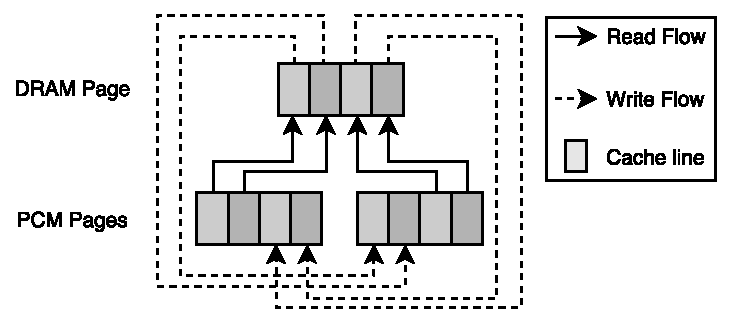
\includegraphics[width=\columnwidth]{page_mapping}
%     \caption{Twins Page Mapping[obsolete]}
% \label{fig:page_mapping}
% \end{figure}

Checkpointing period is to gather all checkpoint related information and construct a checkpoint.
During this period, application will be suspended until checkpoint is established.
Prior works propose to pre-copy checkpoint during execution period~\cite{kannan_optimizing_2013, gao_real-time_2015}, so that checkpointing could overlaps with execution partially and application will suspend for a shorter time.
Such optimization also works for our checkpointing system and can be ported in easily.
However, this paper tries to focus on using Twins Page Mapping to overcome the checkpoint consistency problem, thus we use a simple model without pre-copy optimization here.

\subsection{Twins Page Mapping}\label{sec:page_mapping}

\begin{figure}
    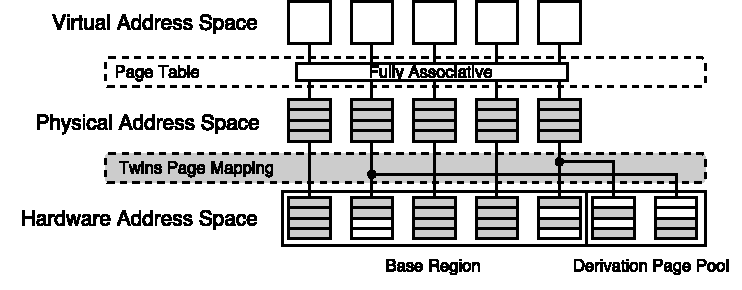
\includegraphics[width=\columnwidth]{page_mapping_2}
    \caption{Twins Page Mapping}
\label{fig:page_mapping}
\end{figure}

Twins Page Mapping is a fine-grained address remapping mechanism aims to resolve the checkpoint consistency problem.
It has a paired page to store
It is a hardware mechanism that targets to translate physical address to hardware address.
Physical address is the address space which can be observed by operating system, while hardware address is independent for different mediums.
For example, if a PCM page is cached in DRAM, these two pages share same physical address, but their hardware addresses vary.

We first introduce two observations, which inspire Twins Page Mapping.
\begin{enumerate*}
    \item Fine-grained address remapping mechanism can resolve checkpointing consistency problem with little extra writes.
		As the analysis in Section~\ref{sec:motivation-in_memory_checkpointing}, logging has at least 1x extra writes.
		These extra writes have stable count and are hard to avoid.
        In contrast, the extra writes caused by copy-on-write is variable.
        Figure~\ref{fig:modifies} shows that averagely 51.3\% of the writes are extra.
        In other words, page-level copy-on-write incurs about 1x more extra writes than cache line-level copy-on-write on average.
        So reduce the granularity of copy-on-write can reduce extra writes.
        Since the granularity of copy-on-write is determined by address remapping mechanism, we conclude that fine-grained address remapping mechanism could help reducing extra writes.
	% \item Fine-grained address remapping mechanism should be an efficient solution for checkpoint consistency problem.
    %
    %     Copy-on-write is based on address remapping mechanism.
    %     Fine-grained copy-on-write requires fine-grained address remapping mechanism
    %
    %
	% 	As the analysis in Section~\ref{sec:motivation-in_memory_checkpointing}, logging has at least 1x extra writes.
	% 	These extra writes have stable count and are hard to avoid.
    %     In contrast, copy-on-write has the potency to achieve 0 extra write.
    %     A typical copy-on-write has three steps.
    %     First, copy old data to new area.
    %     Second, update new area with new data.
    %     Third, change page mapping.
    %     If all data has been modified, we can replace the first two steps with one step that write new data to new area.
    %     In this situation, copy-on-write achieves it best performance and incurs 0 extra write.
    %     Actually, such copy-on-write is address remapping mechanism.
    %
    %     It remaps the virtual address to new area, so write request is redirected to new area.
    %
    %     It just remaps physical address to a new hardware address and this new hardware address handles the write request.

        % This situation is rare as our evaluation showed in Figure~\ref{fig:modifies} under the granularity of page.
        %
        % However, this situation is rare as our evaluation showed in Figure~\ref{fig:modifies} under the granularity of page.
        % Reduce the granularity makes this situation be more possible.
        % So fine-grained copy-on-write should be efficient.
        %
        % The maximum size of possible extra write is the same as the granularity, so smaller granularity mitigates this problem.
        % Actually, such copy-on-write is address remapping mechanism.
        % It just remaps physical address to a new hardware address and new area
        % However, this situation is rare as our evaluation showed in Figure~\ref{fig:modifies} under the granularity of page.
        % The maximum size of possible extra write is the same as the granularity, so smaller granularity mitigates this problem.
        %
        % If all cache lines of a page has been modified, we can replace the first two steps with write new data to new area.
        % Then we achieve 0 extra write.
        %
        % In contrast, the extra writes caused by copy-on-write vary from 1x to 64x (suppose only a 64 bytes of cache line in a 4096 bytes of page is modified) theoretically.
        % So it has the potency to achieve 0 extra writes.
        % Such 0 extra writes situation happens if all cache lines of a page have been modified.
        %
        % These are two possible ways to achieve such high performance.
        % One is that make sure every cache lines in a page have been modified.
        % But as our evaluation showed in Figure~\ref{fig:modifies}, this situation is rare.
        % The other way is fine-grained copy-on-write.
        % The copy process of cache line-level copy-on-write and following data update happen on the same address, so copy process can be skipped.
        %
        % The maximum size of possible extra write is the same as the granularity of copy-on-write, so smaller granularity mitigates this problem.
        % However, reduce the granularity of copy-on-write requires incurs unacceptable overhead.
		% For every page, cache line-level copy-on-write needs 2688 bits of cache line index while page-level copy-on-write only needs 32 bits of page index.
		% The metadata required is too large to accept.
    \item For fault tolerance, older checkpoints can be dropped when a new checkpoint is established\cite{rajachandrasekar_1_2013}.
		Checkpoint used for fault tolerance is to recover application to latest executable state after failure happens.
        So we only need to keep two versions of data in memory, namely latest checkpoint and working memory.
		% So what we need is just the latest checkpoint, and older ones can be dropped.
    % \item Memory-based checkpointing is just changing the role of working memory to checkpoint.
    %     So checkpoint has the same address as working memory of last interval.
\end{enumerate*}

The first observation inspires us to design a fine-grained address remapping mechanism.
General-purpose fine-grained address remapping mechanism incurs large overhead because it needs to be able to map physical address to any hardware addresses.
However, the second observation inspires us that a checkpointing-dedicated address remapping mechanism only needs to map a physical address to two specific hardware addresses, one of which stores checkpoint and the other one stores working memory.
This gives us a chance to design a feasible fine-grained address remapping mechanism.

% The copy and update process of cache line-level copy-on-write happen on the same address and can be merged to one operation.
% It is similar with remapping physical address to another hardware address and writing updated data.
% So a fine-grained address remapping mechanism should be as efficient as fine-grained copy-on-write.

% The second observation inspires us that since checkpointing only needs to maintain two versions of data, namely latest checkpointing and working memory, we can restrict that a physical address can only be mapped to two hardware addresses.
% One of these two hardware addresses stores checkpoint, and the other one stores working memory.
% This restriction gives us a chance to use less metadata than general-purpose address remapping mechanism.

Based on these two observations, we propose a checkpointing-dedicated address remapping mechanism, called Twins Page Mapping.
Twins Page Mapping maps one physical page with two hardware pages.
It restricts that the $n_{th}$ cache line of physical page can only be mapped to the $n_{th}$ cache line of these two hardware pages.
So every cache line of physical page only needs one bit to indicate which hardware page should it be mapped to.
The metadata required by Twins Page Mapping is much smaller than general-purpose fine-grained address remapping mechanism and makes it more feasible.

% Twins Page Mapping maps one physical page ($P$) with two hardware pages ($H1$ and $H2$).
% It restricts that the $n_{th}$ cache line of $P$ ($P_n$) can only be mapped to the $n_{th}$ cache line of $H1$ ($H1_n$) and $H2$ ($H2_n$).
%
% Suppose $H1_n$ stores checkpoint, then any memory access request of $P_n$ should be redirected to $H2_n$ to avoid the modification of checkpoint.
% After checkpointing, $H1_n$ and $H2_n$ exchange roles.
% $H2_n$ becomes checkpoint, and $P_n$ is mapped to $H1_n$.
% Since $P_n$ only has two candidate hardware addresses, namely $H1_n$ and $H2_n$, and these two candidate hardware addresses are not changed after checkpointing, every cache line of physical page only needs one bit to indicate which one of these two candidate hardware address stores checkpoint.

Figure~\ref{fig:page_mapping_example} presents an example of using Twins Page Mapping to keep checkpoint consistent.
To explain the behaviors of Twins Page Mapping in different situations, we select four points in time from the first four consecutive periods respectively.
We assume that a page is composed by four cache lines in this example.
\begin{enumerate*}
    \item
        The first one is arbitrary time during initial execution period.
        During initial execution, every physical page maps with one hardware page, which is called \textit{Base Page}.
        The physical address of physical page should be the same as the hardware address of Base Page.
        At this time, Base Page stores working memory and services memory request as normal memory system.
    \item
        The second point is the end of first checkpointing.
        All data is marked as checkpoint.
        So they have two roles now, namely checkpoint and working memory.
    \item
        The third point is some time after application resumes execution.
        During execution, every read request is intercepted and redirected to working memory.
        Write request is also intercepted, but it needs more attention from Twins Page Mapping.
        Twins Page Mapping first checks whether this physical page has been mapped with two hardware pages.
        If not, Twin Page Mapping will allocate a new hardware page, which is called \textit{Derivation Page}, and establishes the mapping relation.
        Then Twins Page Mapping translates physical address in terms of the role of data.
        Suppose a request tries to write the $n_{th}$ cache line of physical Page.
        Twins Page Mapping finds that the $n_{th}$ cache line of Base Page has the role of checkpoint, so it translates the address to the $n_{th}$ cache line of Derivation Page.
        Thus checkpoint keeps unmodified.
        The role of data also changes.
        Before such write, $n_{th}$ cache line of Base Page has two roles of checkpoint and working memory.
        But after write, $n_{th}$ cache line of Base Page only has one role of checkpoint, while the $n_{th}$ cache line of Derivation Page will be given a role of working memory.
    \item
        The fourth point is the end of second checkpointing.
        All data only has one role of checkpoint is part of the checkpoint generated by last interval.
        So we drop them and mark them as unused.
        Except the data which is unused, rest data has the role of working memory.
        They are part of the checkpoint generated by this interval, so they will be given the role of checkpoint, too.
\end{enumerate*}

% Figure~\ref{fig:page_mapping_example} elaborates a sample flow of Twins Page Mapping.
% At first, every physical page is mapped to one hardware page, which is called \textit{Base Page}.
% After the first checkpointing, all data is marked as both working memory and checkpoint.
% Then application resumes execution and try to write memory.
% The write request causes an allocation of new hardware page, which is called \textit{Derivation Page}.
% All memory write request will be redirected to Derivation Page.

% Twins Page Mapping first maps one physical page ($P$) with two hardware pages ($H1$ and $H2$).
% Then it restricts that the $n_{th}$ cache line of $P$ ($P_n$) can only be mapped to the $n_{th}$ cache line of $H1$ ($H1_n$) and $H2$ ($H2_n$).
% Suppose $H1_n$ stores checkpoint, then any memory access request of $P_n$ should be redirected to $H2_n$ to avoid the modification of checkpoint.
% After checkpointing, $H1_n$ and $H2_n$ exchange roles.
% $H2_n$ becomes checkpoint, and $P_n$ is mapped to $H1_n$.
% Since $P_n$ only has two candidate hardware addresses, namely $H1_n$ and $H2_n$, and these two candidate hardware addresses are not changed after checkpointing, every cache line of physical page only needs one bit to indicate which one of these two candidate hardware address stores checkpoint.

% To be specific, we explain how our fine-grained checkpointing-dedicated address remapping mechanism works in Figure~\ref{fig:page_mapping_example}.
% To be specific, our fine-grained checkpointing-dedicated address remapping mechanism, which is called Twins Page Mapping, first maps one physical page with two hardware pages (called \textit{Base Page} and \textit{Derivation Page}).
% Then it restricts that the $n_{th}$ cache line of the physical page can only be mapped to the $n_{th}$ cache line of Base Page or Derivation Page.
% Suppose that the $n_{th}$ cache line of Base Page stores checkpoint, any memory access request will be redirected to the $n_{th}$ cache line of Derivation Page to keep checkpoint data consistent.
% After checkpointing, the roles of these two addresses exchange.
% The $n_{th}$ cache line of Derivation Page becomes checkpoint, and future memory access request are going to be redirected to Base Page.
% Because every cache line of physical page only has two candidate hardware addresses, every cache line only needs 1 bit to indicate which hardware page contains checkpoint.
% This restriction reduces the size of metadata substantially and makes Twins Page Mapping be more feasible than fine-grained copy-on-write.

% [to modify]
% As described in Section~\ref{sec:design_overview}, \textit{Twins Page Mapping} maps one DRAM page with two PCM pages.
% At first, every DRAM page maps with one PCM page, just like normal hybrid memory systems.
% We call this PCM page \textit{Original Page}.
% Then we may request for a new PCM page to build Twins Page Mapping along with the system processing.
% This new PCM page is called \textit{Derivation Page}.

\begin{figure}
    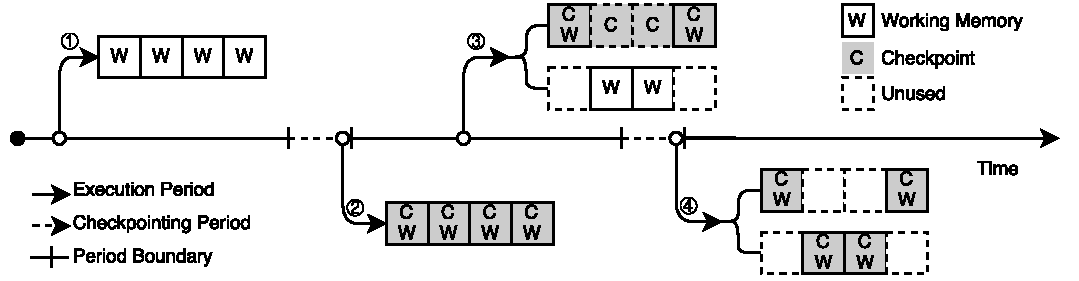
\includegraphics[width=\columnwidth]{page_mapping_example}
    \caption{An Example of Using Twins Page Mapping to Keep Checkpoint Consistent.
        We suppose a page with four cache lines.
        \circled{1} During initial execution period, all data is working memory.
        \circled{2} At the end of first checkpointing period, all data becomes checkpoint.
        \circled{3} In the period of second execution, any write to checkpoint will trigger the allocation of Derivation Page.
            Write request will be redirected to corresponding cache line which does not stores checkpoint.
            Then such checkpoint data will have only one role of checkpoint, and the corresponding cache lines will be given a role of working memory.
        \circled{4} When second checkpointing period ends, working memory becomes checkpoint and other data is dropped.
    }
\label{fig:page_mapping_example}
\end{figure}

\subsection{Coordinating with Hybrid Memory System}

\subsubsection{Avoid Intercepting All Memory Requests}

% \textbf{Reduce Address Translation.}
Intercepting all memory requests to check or even translate address could potentially slow down system, especially for memory-intensive applications.
Hybrid memory system helps to mitigate this problem.
Coordinating with hybrid memory system, Twins Page Mapping only intercepts the memory requests happen on PCM, that is memory requests caused by cache miss and checkpointing.
Because the high performance of hybrid memory system has been proved by prior works, we could expect a relative low probability of cache miss.
So most of memory requests will hit DRAM and be serviced by DRAM directly without performance lost.

% To achieve high performance, Twins Page Mapping has to address an obstacle, which is the overhead incurred by metadata.
% Metadata overhead is critical for Twins Page Mapping because of two reasons.
% First, we have to access metadata before any memory access request.
% Twins Page Mapping should redirect memory access request to working memory so that it can avoid the modification on checkpoint.
% This feature enforces us to read metadata before any memory access request to identify the address of working memory, and leads massive accesses of metadata.
% Although memory controller is fast, massive access still incurs high overhead.
%
% We coordinate with hybrid memory system and only read metadata during cache replacement process.
% Since use DRAM as the cache of PCM has been evaluated as a promising architecture, revisit data should be a common access pattern.
% So compared with aforementioned process, which needs to read metadata before every memory access requests, reading metadata only when cache misses can reduce metadata accesses.
% After cache replacement process, every memory access request is serviced by DRAM directly with low overhead.

\subsubsection{Mitigating Metadata Overhead}\label{sec:design_mitigating_metadata}

Twins Page Mapping restricts that every cache line can only be mapped to two candidates, which leads much less metadata than general-purpose address remapping mechanisms.
However, as we will present in Section~\ref{sec:implementation_metadata}, every page still needs a relative large metadata.
In our evaluation, 1.5MB of metadata is required.
Although DRAM and PCM can afford such storage overhead easily, it is still a burden for memory controller.
To address this problem, we propose to select partial metadata and store them in memory controller.

Memory controller version of metadata contains essential data for two things.
First, like full version of metadata, checking whether requested address has Derivation Page.
Second, indicating the position of only the first several cache lines of page.

To cooperate with this shrinking metadata, we also modify the processes of flushing DRAM page and caching PCM page.
To introduce the impact of our modified processes, we first present a simplified ideal page access process model in Figure~\ref{fig:tag_access}a.
If memory controller is large enough for all metadata, we could read metadata from memory controller, and then following the indication of metadata to read cache lines from DRAM or PCM\@.
The whole latency of read multiple cache lines generally is not the sum of each cache line's read latency.
Further cache line access process could be accelerated by several mechanisms, such as bank-level or rank-level parallel, accessing an opened row etc.
To keep our page access process model simple, we mark all these mechanisms as parallel.

Flushing DRAM page in our system involves three steps.
First, accessing memory controller to check whether we need more metadata.
If the requested address has no Derivation Page, we could access DRAM normally.
Otherwise we should perform second step, which is acquiring full version of metadata from DRAM\@.
Third, reading cache lines from DRAM and writing them back to PCM\@.
This modified process costs more time than ideal page access model because we need to read metadata from DRAM before performing real cache line read.
However, this should not be a problem for our system.
We explain it by analyzing two scenes of flushing DRAM page.
\begin{enumerate*}
    \item Cache miss during execution phase.
        As Figure~\ref{fig:dram_pcm_busy_time} [not in this paper now] presents, because we use a quite small checkpointing interval, most of pages would be flushed by checkpointing instead of cache miss.
        Hence although flushing DRAM page incurs delay, the low frequency makes this overhead negligible.
    \item Checkpointing phase.
        Flushing process contains two parts, namely read data from DRAM and write data to PCM\@.
        DRAM read latency is much smaller than PCM write latency, so before PCM finishes a write request, DRAM could have finished read and send this data to PCM's write queue.
        Figure~\ref{fig:dram_pcm_busy_time} [not in this paper now. same figure as last missing one] proves this analysis.
        It shows that the critical path of checkpointing is composed by several DRAM read requests and lots of PCM write requests.
        As a result, checkpointing phase is also only delayed by several DRAM read requests.
        % Thus most of DRAM read is not on critical path of checkpointing.
        % This is because of two reasons.
        % First, checkpointing process performs flushing intensively and continuously.
        % Second, DRAM read latency is much smaller than PCM write latency.
\end{enumerate*}

Caching PCM page contains four steps in our system.
First, we also access memory controller to get memory controller version of metadata.
Second, following the indication of such metadata, we start reading the first several cache lines from PCM instantly.
Third, at the time of reading cache lines from PCM, read DRAM to get a full version of metadata.
Fourth, perform rest memory access when we got the full version of metadata.
Because read latency of PCM is several times larger than DRAM, and DRAM and PCM could perform read operation concurrently, we could expect that the third step will finish before the second step.
If so, the fourth step will start without delay.
Hence our caching PCM page process has the potential to gain same performance as ideal page access model.

\begin{figure}
    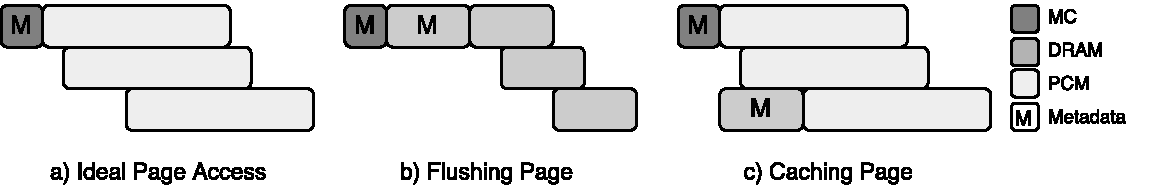
\includegraphics[width=\columnwidth]{tag_access}
    \caption{Page Access Process}
\label{fig:tag_access}
\end{figure}

\section{Implementation}\label{sec:implementation}

In this section, we propose the implementation details of our checkpointing system.
At first, we introduce the metadata management of Twins Page Mapping, followed by the details of page movement between DRAM and PCM\@.
Then Derivation Page management is presented.
At last, we introduce the checkpointing process.

\subsection{Metadata Management}\label{sec:implementation_metadata}

Metadata of Twins Page Mapping is maintained in a table called Derivation Page Table (DPT).
The columns of DPT is:
\begin{enumerate*}
    \item A 36 bits of Base Page Index which stores the higher-order bits of Base Page's physical address.
    \item A 64 bits of Checkpoint Position indicating that whether checkpoint is stored in Base Page or Derivation Page.
        Every bit represents a cache line.
    \item A 2 bits of Working Memory Position.
        Its usage is similar like Checkpoint Position, which is indicating whether working memory is stored in Base Page or Derivation Page.
        However, it only has two bits to represent the position of the first two cache lines.
        Its usage has been explained in Section~\ref{sec:design_mitigating_metadata}.
    \item A 64 bits of Physical Page Dirty indicating that whether the cache line of physical page has been modified since last checkpointing.
\end{enumerate*}

% Every Derivation Page should have an entry in DPT\@.
% So the size of DPT is determined by the count of candidate Derivation Pages.

% We maintain two versions of DPT and place them on PCM and DRAM respectively.
% These two versions of DPT has different purposes, so the columns in them also vary, as listed in Table~\ref{tbl:metadata}.
% Utilizing the persistent feature of PCM, we store a version of DPT in PCM for recovery after system failure.
% The other version of DPT is stored in DRAM for performance concern.
% Besides that, it is also used to store Physical Page Dirty, which assists locating working memory but is useless for recovery.

We maintain three versions of DPT and place them in memory controller, DRAM and PCM respectively.
These three versions of DPT have different purposes, so the columns of them also vary, as listed in Table~\ref{tbl:metadata}.
Memory controller version of DPT aims to be small so it can be hold by memory controller.
It has two columns, namely Base Page Index, and Working Memory Position.
For DRAM version of DPT, size is not the problem.
It stores all columns except Working Memory Position and provides efficient access.
PCM version of DPT is for recovery.
Thus it only takes essential columns, i.e. Base Page Index and Checkpoint Position.

% \begin{table}
%     \renewcommand{\arraystretch}{1.3}
%     \caption{DPT columns}
% \label{tbl:metadata}
%     \centering
%     \begin{tabular}{| c | >{\centering\arraybackslash} m{2.55cm} | >{\centering\arraybackslash} m{2.4cm} | >{\centering\arraybackslash} m{1.5cm} |}
%         \hline            & Base Page Index   & Checkpoint Position   & Physical Page Dirty   \\
%         \hline Size       & 36 bits           & 64 bits               & 64 bits               \\
%         \hline Version    & Memory Controller \& DRAM \& PCM        & DRAM \& PCM                     & DRAM                     \\
% 	\hline
%     \end{tabular}
% \end{table}

\begin{table}
    \renewcommand{\arraystretch}{1.3}
    \caption{DPT columns}
\label{tbl:metadata}
    \centering
    \begin{tabular}{| c | >{\centering\arraybackslash} m{1.3cm} | >{\centering\arraybackslash} m{1.3cm} | >{\centering\arraybackslash} m{2cm} | >{\centering\arraybackslash} m{1.3cm} |}
        \hline                      & Base Page Index   & Checkpoint Position & Working Memory Position   & Physical Page Dirty   \\
        \hline MC                   & 36 bits        & -                 & 2 bits   & -                     \\
        \hline DRAM                 & 36 bits        & 64 bits           & -        & 64 bits           \\
        \hline PCM                  & 36 bits        & 64 bits           & -        & -                     \\
	\hline
    \end{tabular}
\end{table}

To reduce PCM writes, we also adopt a common optimization that only write dirty cache lines~\cite{qureshi_scalable_2009, ham_disintegrated_2013}.
This optimization requires a 64 bits of tag, called DRAM Page Dirty, for every dram page.
This tag indicates whether the cache lines of dram page have been modified since they were read into DRAM\@.
Because such tag can be used for different purposes and is so common (cite), we expect it could become the standard of future hybrid memory system.
Hence it is excluded from overhead caused by our design.

% Memory controller version of DPT can only be used to check whether physical address hits DPT\@.
% Further usage of DPT, such as indicating which cache line should be visited, requires to access DRAM to acquire a full version entry.
% Inserting a DRAM read before every PCM access request seems to slow down system.
% However, hybrid memory system helps mitigating this concern, and the details will be presented in next section.

% However, our evaluation on Section~\ref{sec:evaluation_metadata} proves that it can only produce negligible overhead.

% [TODO] The size of metadata is important for system performance.

% This memory controller version of DPT reduces 78\% of metadata size and our evaluation (Section~\ref{sec:evaluation_metadata}) will show that read full entry from DRAM will not be a big problem for system performance.
% To address this problem, we propose to construct a memory controller version of DPT by 36 bits of Base Page Index, 4 bits of Checkpoint Position and 4 bits of Physical Page Dirty.
% Through this optimization, we reduce 73.2\% of metadata requirement.
%
% We then analysis why such optimization will be efficient.
% As we only read metadata when flush DRAM page to PCM or read PCM page to DRAM, we elaborate this optimization from these two aspects.
%
% \textbf{Read PCM page.}
% Read PCM page is quite simple.
% We just do it as normal.

\subsection{Page Movement Between DRAM and PCM}\label{sec:implementation_hybrid_memory_system}

% Since hybrid memory system is a promising trend, we choose it as our target system.
% In return, it also helps us to avoid intercepting all memory requests and mitigate metadata overhead.

% Data stored in DRAM can service memory requests directly.
% Only those memory requests which needs to access PCM will be intercepted by Twins Page Mapping.
% During execution, such memory requests only appear when cache misses.

There are two possible ways to trigger page movement between DRAM and PCM\@.
The first one is cache miss.
A typical cache replacement process contains three steps.
\begin{enumerate*}
    \item Choosing victim page according to cache replacement algorithm.
    \item Flushing the data stored in victim page to corresponding PCM page.
    \item Copying data from expected PCM address to victim page.
\end{enumerate*}
The latter two steps are replaced with the \textbf{Divide} and \textbf{Merge} process of Twins Page Mapping respectively.
The second one is checkpointing.
Checkpointing needs to flush DRAM pages to PCM\@.
This process can also be replaced by \textbf{Divide} process.

\textbf{Divide} will divide DRAM page by cache line and write these cache lines to corresponding PCM pages.
As Figure~\ref{fig:divide_and_merge} illustrates, we first update tag Physical Page Dirty by bitwise OR it with DRAM Dirty.
% Then we calculate a temporary tag $T = Physical\ Page\ Dirty \oplus Checkpoint\ Posisiton$.
% we first update tag Physical Page Dirty by Equation~\ref{eq:logical_page_dirty_update}.
Then we calculate a temporary tag $P$ by Equation~\ref{eq:tmp_tag_in_twin_page}.
The value of $P$ indicates the position of working memory.
Suppose the $n_{th}$ bit of $P$ is 0, the $n_{th}$ cache line of physical page will be translated to the $n_{th}$ cache line of Base Page.
Otherwise it will be translated to the $n_{th}$ cache line of Derivation Page.
% If cache line is dirty, it is written to specific PCM address indicated by $TAG_{tmp\ checkpoint\ position}$ to avoid overwriting old data.
In addition, we only write dirty cache lines to reduce writes.

\begin{equation}
    P = Physical\ Page\ Dirty \oplus Checkpoint\ Posisiton
\label{eq:tmp_tag_in_twin_page}
\end{equation}

% \begin{equation}
%     DIRTY_{physical} = DIRTY_{physical} \lor DIRTY_{dram}
% \label{eq:logical_page_dirty_update}
% \end{equation}
%
% \begin{equation}
%     POSITION_{tmp} = POSITION \oplus DIRTY_{physical}
% \label{eq:tmp_tag_in_twin_page}
% \end{equation}

\textbf{Merge} selects cache lines from Base Page and Derivation Page according to the indication of metadata, and then merges them to an intact page in DRAM\@.
Figure~\ref{fig:divide_and_merge} illustrates this process.
Merge process is simpler than Divide.
We just need to calculate a temporary tag $P$ by Equation~\ref{eq:tmp_tag_in_twin_page}.
Then we could read cache lines following the value of $P$ and write them to DRAM\@.
At last, we get a normal DRAM page which can be accessed directly.
% We first calculate a temporary tag $TAG_{tmp\ in\ twin\ page}$ like Divide process.
% Then we read cache lines from PCM according to this tag.
% At last, we write these cache lines to DRAM so that a DRAM page is composed.

\begin{figure}
    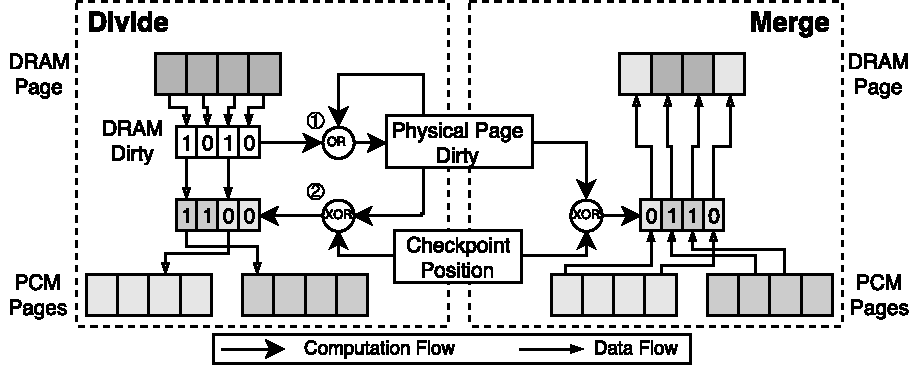
\includegraphics[width=\columnwidth]{dram_and_pcm}
    \caption{Divide and Merge Processes of Twins Page Mapping}
\label{fig:divide_and_merge}
\end{figure}


% \begin{figure}
%     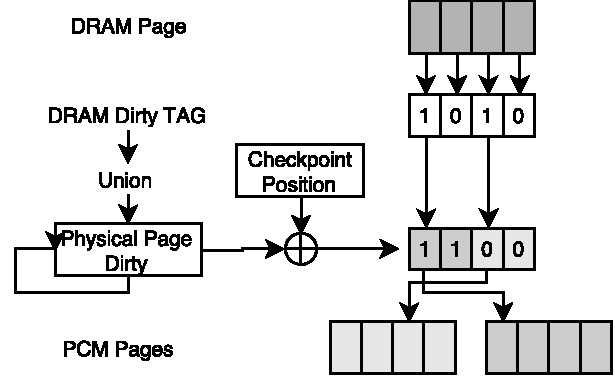
\includegraphics[width=\columnwidth]{dram_to_pcm}
%     \caption{Divide Operation of Twins Page Mapping}
% \label{fig:dram_to_pcm}
% \end{figure}
%
%
% \begin{figure}
%     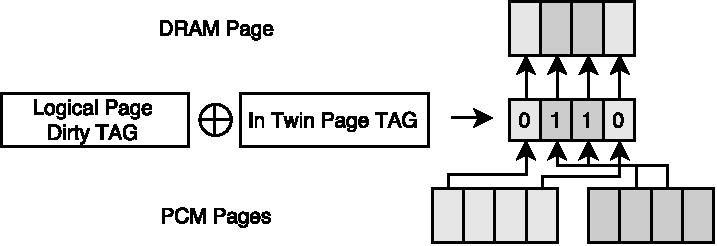
\includegraphics[width=\columnwidth]{pcm_to_dram}
%     \caption{Merge Operation of Twins Page Mapping}
% \label{fig:pcm_to_dram}
% \end{figure}

% Besides of cache miss, Twins Page Mapping also works during checkpointing.
% Checkpointing uses Divide process to persist data stored in DRAM\@.

Note that, the tag update of Divide and Merge process all happens on the DRAM version of DPT\@.
We do this for two reasons.
First, update DRAM version of DPT can benefit from the high performance of DRAM\@.
Second, and also the key reason, these update helps to locate the position of working memory but has no effect for checkpoint.
So persisting them to PCM makes no sense.

\subsection{Derivation Page Management}\label{sec:page_pool}

\subsubsection{Derivation Page Pool}

% We propose two alternative ways to manage Derivation Pages, which are fixed space method and dynamic space method.

% \textbf{Fixed Space:}

Derivation Page Pool is the structure used for storing Derivation Pages.
It is a reserved large and continuous PCM area, and is managed by hardware.
We split it into multiple pages and use bitmap to record whether a page a allocated.
% It only supports one kind of request, that is Derivation Page Allocation.

% We reserve a continuous PCM area as the to service the allocation of Derivation Pages.
% This area is called \textit{Derivation Page Pool}.
% Derivation Page Pool splits itself into multiple pages and uses bitmap to record whether a page is allocated.
% It only services one kind of request, Derivation Page Allocation.

% Fixed space method only responses page allocation request.
% Page release request is just ignored.

% \textbf{Dynamic Space:} Dynamic space method relies on page management of operating system.
% It just forwards page allocation and release request to operating system.
% So dynamic space method is more flexible but less efficient.
% When operating system releases pages, dynamic space method adds theses pages to a list called \textit{pages\_to\_free}, and they will not be allocated again during this checkpointing.
% We can not release them immediately because checkpoint data is stored in there.
% At the end of final checkpointing, every logical page in \textit{pages\_to\_free} list will be called by Revoke Mapping operation to release Derivation Page.
% Meanwhile, original page is also released.

The size of Derivation Page Pool is important.
It determines the size of DPT, so a large Derivation Page Pool aggravates the overhead of metadata.
However, small Derivation Page Pool leaves a high possibility of failing to find a free Derivation Page.
So we perform an experiment in Section~\ref{sec:evaluation_storage_overhead} to evaluate the influence of different size of Derivation Page Pool.

\subsubsection{Allocating Derivation Page}

To service Derivation Page Allocation request, we first scan the bitmap of Derivation Page Pool and try to find a free page.
If a free page is found, we return this page to caller.
Otherwise, we would try to release a Derivation Page and return it to caller.
If we fail again, we should call checkpointing to get releasable pages.

Derivation Page Allocation is requested during execution.
At the end of checkpointing interval, all PCM pages are marked as write-protect.
In next execution period, any write to these write-protect pages will trigger a check of mapping state.
If mapping is not established, we will send a Derivation Page Allocation request to Derivation Page Pool.

Note that, the write to DRAM page, but not the write to PCM page, will trigger Derivation Page Allocation.
An integrate checkpointing process make all pages clean and ready to be released.
So calling checkpointing is the last resort to meet the allocation requirement of caller, and we have to ensure that we can finish an integrate checkpointing process under any situation.
This requirement results that allocating Derivation Page when a write happens on PCM is not appropriate.
If we fail to allocate a Derivation Page to service a PCM write, we could not expect checkpointing, which will incurs more PCM writes, can finish smoothly.
In contrast, allocate Derivation Page when we write to DRAM ensures that all dirty DRAM pages have allocated Derivation Page.
So write back can be processed without failure.
As a result, we can processing an integrate checkpointing at any time.

\subsubsection{Releasing Derivation Page}

To release space, we first scan Derivation Page Pool to find a releasable page.
A releasable page is such a page that
\begin{enumerate*}
    \item its Physical Page Dirty tag is cleared, which means it has not been modified during this checkpointing interval.
    \item if it is cached in DRAM, corresponding DRAM page should be clean.
\end{enumerate*}
These two condition ensures that it only has one version of data stored in memory, namely last checkpoint.
So we can extract the data belonged to last checkpoint from Derivation Page and write it to corresponding cache lines of Base Page.
Then Derivation Page can be freed.

If Derivation Page Pool can not find such a page, which means all pages have been modified during this checkpointing interval, Derivation Page Pool has to tell caller that Page Allocation fails.
Caller should call checkpointing instantly to get some releasable pages and request for Derivation Page Allocation again.

Derivation Page Release should never be requested by caller proactively because Derivation Page is released automatically when we can not find a free page for allocation.
This design keeps operating system's page management transparent for hardware, which reduces the communication between operation system and hardware, and also simplifies system.

\subsection{Checkpointing}

Checkpointing needs to persist three kinds of data, namely working memory, CPU context information and DPT\@.
In this section, we will explain the checkpointing processes of these data respectively.

During execution, cache eviction has moved partial working memory to PCM\@.
Thus what left for checkpointing period is flushing data stored in DRAM to PCM\@.
To be specific, we will call Divide process for all dirty DRAM pages.

Checkpointing is triggered by application or operating system proactively.
So application or operating system is responsible to determine the composition and the store address of CPU context information.
To avoid failure during checkpointing, such data should be stored in different address with previous checkpoint.

Before we persistent DPT, we need to update it first.
This involves three steps.
First, we update Physical Page Dirty by bitwise OR it with DRAM Dirty.
Second, we update Checkpoint Position by bitwise XOR it with Physical Page Dirty.
Third, the new PCM version of DPT, which is composed by Physical Page Dirty and Checkpoint Position are written to PCM\@.
Certainly, they will also be written to a different address with previous checkpoint to avoid failure during checkpointing.

Besides of persisting data, we also need to prepare for resuming application.
We need to reset Physical Page Dirty and DRAM Dirty.
And the DRAM version of DPT should be overwritten by corresponding columns of PCM version of DPT\@.
Eventually, we establish a checkpoint and are ready to resume application.
Checkpointing period ends.

% \subsection{Recovery}

% \subsection{Discussion}\label{sec:discussion}
%
% For application running in hybrid memory system, Twins Page Mapping will reduce available memory.
% In the worst case, all data is modified between two subsequent checkpointing.
% Half of the memory will be application data and the rest are checkpoint data generated by last checkpointing.
% However, reduce checkpointing interval will absolutely relieves this situation.
% A smaller checkpointing interval reduces the data changed between two checkpointing and increases the reliability of system.
%
% Lazy checkpointing is effected by two prediction algorithms, namely prediction of idle period and prediction of data going to be written.
% A more accurate idle period prediction algorithm will reduces the time which blocks application, while a more precise prediction of data going to be written guides us to avoid sync trigger by write.
% Consequently, better prediction algorithms from other works will help improve the performance of lazy checkpointing.

\section{Evaluation}\label{sec:evaluation}

Our evaluation tries to answer following questions:
\begin{enumerate}
    \item How does our system perform overall?
    \item What is the storage overhead and how does different storage overhead affect system performance?
    \item Does our system slow down if we only store partial metadata in memory controller?
\end{enumerate}

% In this section, we first introduce experimental methodology, then detailed evaluation is presented.

\subsection{Experimental Methodology}\label{sec:evaluation_methodology}

\subsubsection{Experimental Platform}

We build our experimental environment using MARSSx86\cite{patel_marss_2011}, a full system simulation tool for x86-64 architecture. % chktex 8
A quad-core system which has out-of-order core pipeline is conducted.
Every core has a frequency of 1.87 GHz and 128KB of L1 I/D cache.
A 2MB of L2 cache is shared by all cores.

Memory system is consisted of DRAM and PCM\@.
DRAM is a 256MB DDR3 device simulated by DRAMSim2\cite{rosenfeld_dramsim2_2011}, while PCM is simulated by NVMain\cite{poremba_nvmain_2015} with a size of 8GB\@.
They both adopt the timing parameters presented by~\cite{lee_architecting_2009}, such as tRCD, tCL, tRP etc.
HybridSim\cite{stevens_integrated_2013} integrates DRAM and PCM\@.
It takes DRAM as the cache of PCM, and uses classical LRU as cache replacement algorithm.

\subsubsection{Comparison}

We compare with two memory-based checkpointing systems, which use logging and copy-on-write to resolve checkpointing consistency problem respectively.
\begin{itemize}
    \item \textit{Logging} accesses data by the granularity of cache line.
        It copies old data to log area first before writes new data.
        To gain a better performance, we adopt a optimization from~\cite{sorin_safetynet_2002} that only log for the first modification per checkpointing interval.
    \item \textit{Copy-on-Write} copies data to new page and redirects further memory access requests to new page.
        Such process happens only at the time of cache misses.
        We adopt two optimization for copy-on-write.
        First, address remapping mechanism is maintained by memory controller.
        Second, we reserve a large enough space to ensure that new page allocation can always be satisfied and can be finished by hardware.
    % \item The other one is Mona, which is one of state-of-the-art PCM-assisted Checkpointing systems.
    %     Mona is also implemented in hybrid memory system.
    %     Load balancing of Mona can be ported to our system, so we focus on the comparison with Mona's partial checkpointing.
\end{itemize}
These two memory-based checkpointing systems have the same configuration as our system.
Memory requests are also handled by DRAM\@.
And if write back does not incurs logging or copy-on-write, only dirty cache lines are written back.

\subsubsection{Workloads}

\begin{table}[!t]
    \renewcommand{\arraystretch}{1.3}
    \caption{Workloads}
\label{tbl:workloads}
    \centering
    \begin{tabular}{|>{\centering\arraybackslash} m{0.6cm}|>{\centering\arraybackslash} m{3.65cm}|>{\centering\arraybackslash} m{1.7cm}|>{\centering\arraybackslash} m{1.1cm}|}
        \hline      & \bfseries Workload             & \bfseries L3 Miss Rate   & \bfseries FP (MB)  \\
        \hline WD1  & gamess h264ref h264ref povray  & 2.0\%                    & 34 \\
        \hline WD2  & bzip2 bzip2 gromacs gromacs    & 24.2\%                   & 1716 \\
        \hline WD3  & bzip2 gcc gromacs perlbench    & 40.4\%                   & 1842 \\
        \hline WD4  & gcc gcc mcf perlbench          & 57.3\%                   & 2471 \\
        \hline WD5  & astar gobmk mcf omnetpp        & 64.7\%                   & 2109 \\
        \hline WD6  & gobmk leslie3d omnetpp wrf     & 77.7\%                   & 986 \\
        \hline WD7  & leslie3d sjeng sphinx3 wrf     & 88.3\%                   & 1011 \\
        \hline WD8  & GemsFDTD lbm milc soplex       & 96.3\%                   & 1878 \\
        \hline
    \end{tabular}
\end{table}

To evaluate our system's performance, we carefully select applications from SPEC CPU2006\cite{spec2006benchmark} and list them in Table~\ref{tbl:workloads}.
These workloads have evenly distributed L3 cache miss rate~\cite{jaleel_memory_2010} and different footprint, so they can represent a majority of real workloads.
Every workload contains four applications which start simultaneously.
After a warm up phase, we start a simulation for 1.5 billion instructions and request for checkpointing every 30 million cycles.

% These workloads has large footprint to simulate the situation that DRAM is not large enough for future big data application.
% Besides of that, they has different L2 cache miss rate~\cite{jaleel_memory_2010}, which means different locality.
% Memory access patterns of them also varies, so we record the amount of modified cache lines when a page is to be evicted, and show the results in Table~\ref{tbl:workloads}.

% Every workloads contain two applications which start simultaneously.
% After a warm up phase, memory usage stabilizes and simulation starts.
% Simulation lasts for 1.5 billion instructions.
% During simulation, we will request for checkpointing every 200 million cycles.

% We try to answer to questions here.
% \begin{enumerate}
%     \item What's the overall performance?
%     \item How does the size of Derivation Page Pool affect the performance?
%     \item How does checkpointing interval affect the performance?
% \end{enumerate}

% \begin{table}[!t]
%     \renewcommand{\arraystretch}{1.3}
%     \caption{Workloads}
% \label{tbl:workloads_old}
%     \centering
%     \begin{tabular}{|c|c|c|c|c|}
%         \hline & Workload & Miss Rate (Aver) & FP (MB) & Modification \\
%         \hline WD-H & milc, bwaves & 99.8 (High) & 1396 & 11.87 \\
%         \hline WD-M & gcc, mcf & 58 (Middle) & 2478 & 7.89 \\
%         \hline WD-L & bzip2, bzip2 & 20.8 (Low) & 1712 & 62.13 \\
%         \hline
%     \end{tabular}
% \end{table}

\subsection{Overall Evaluation}\label{sec:evaluation_overall}

% \subsubsection{Application Running Time}

\textbf{Workload Execution Time.}
At first, we present the comparison of workload execution time in Figure~\ref{fig:overall_time}.
All results are normalized by our checkpointing system, which is marked as Twins in figures.
A speedup for all workloads are observed.
The average speedup is 1.29x and 1.19x compared with logging and copy-on-write respectively.
For specific workload, we even achieve at most 1.4x and 1.88x speedup.

% We also evaluate the performance of xx-checkpointing without Lazy Checkpointing to evaluate the contribution of Twins Page Mapping.
% XX-checkpointing achieves at most 1.74x speedup compared with PCM-assisted Checkpointing.
% For memory-based Checkpointing, we also gain a speedup of 1.39x$\sim$1.86x.
% In worst situation, which is WD-L, all technologies we test have slight difference.
% WD-L has good locality.
% When a page is to be evicted, 96.8\% cache lines of it have been modified.
% For WD-L, XX-checkpointing only improves system performance of 3\%$\sim$6\%.

% \subsubsection{PCM Write Amount}

\textbf{PCM Write Amount.}
Our another concern is PCM write amount.
Figure~\ref{fig:overall_write} illustrates how much PCM writes are requested during evaluation.
All results are also normalized by our checkpointing system.
As the analysis in Section~\ref{sec:motivation-in_memory_checkpointing}, writes incurred by logging is about 2x, while copy-on-write incurs various write amount for different workloads.
The average PCM write amount of logging and copy-on-write is 1.89x and 4.11x on average.

The performance of Logging and Copy-on-write vary as workload changes.
Logging performs better for WD1, WD3 to WD7, while copy-on-write wins for WD2 and WD8.
The reason for that is the performance of copy-on-write depends on the access pattern of workloads.
Copy-on-write has to copy all pages even if only a small part of it is modified.
So workloads which modifies massive pages but only incurs a spot of modification for each page will perform bad.
In contrast, Twins Page Mapping shows a stable performance for every workloads.
Even for worst case WD1, in which Twins Page Mapping executes same time as logging and copy-on-write, we still observe a clear reduction of PCM writes.

% Low write performance is the key drawback of PCM\@.
% Figure~\ref{fig:overall_write} illustrates how much PCM writes are requested during evaluation.
% All results are also normalized by xx-checkpointing.
% For workloads which have bad locality, fine-grained checkpointing technologies such as Logging-based memory-based Checkpointing and XX-Checkpointing show great performance advantage.
% Mona and Copy-on-Write incur up to 13.54x and 12.41x more PCM writes respectively for WD-H and WD-M.
% In contrast, WD-L has different results.
% For WD-L, Logging incurs 63\% more PCM writes than Copy-on-Write.
% The reason for that is Logging incurs more PCM writes than Copy-on-Write if they deal with the same size data, just like the analysis in Section~\ref{sec:motivation-in_memory_checkpointing}.

\begin{figure}
    \begin{subfigure}{\columnwidth}
        \begin{tikzpicture}
            \begin{axis}[
                height=4cm,
                ybar=0pt,
                ymajorgrids,
                xtick=data,
                xticklabels from table={\LoadOverallTime}{workload},
                xticklabel style={font=\footnotesize},
                ylabel=Execution Time,
                ylabel style={font=\footnotesize},
                % ylabel style={font=\footnotesize, at={(0, 0.3)}},
                enlarge x limits=0.1,
                enlarge y limits={upper, value=0.2},
                ymin=0.85,
                % nodes near coords,
                % every node near coord/.append style={rotate=90, anchor=west, font=\small},
                legend columns = -1,
                legend style={at=({0.5, 1.3}), anchor=north, font=\scriptsize, inner sep=1pt, outer sep=0pt,
                    row sep=0pt},
                legend image post style={scale=0.7},
                legend cell align=right,
                /tikz/every even column/.append style={column sep=0.5cm},
                width=\columnwidth,
                % width=0.7*\columnwidth,
                bar width=5,
            ]
            % \draw[DarkGray, very thin, densely dashed] (axis cs:\pgfkeysvalueof{/pgfplots/xmin},1) -- (axis cs:28,1);
            % \draw[DarkGray, very thin, densely dashed] (axis cs:\pgfkeysvalueof{/pgfplots/xmin},1.2) -- (axis cs:28,1.2);
            % \draw[DarkGray, very thin, densely dashed] (axis cs:\pgfkeysvalueof{/pgfplots/xmin},1.4) -- (axis cs:28,1.4);
                \addplot[fill=LighterGray, area legend] table[x expr=\coordindex, y=page-mapping] \LoadOverallTime;
                \addlegendentry{Twins};
                \addplot[fill=Gray, area legend] table[x expr=\coordindex, y=logging] \LoadOverallTime;
                \addlegendentry{Logging};
                \addplot[fill=DarkerGray, area legend] table[x expr=\coordindex, y=cow] \LoadOverallTime;
                \addlegendentry{Copy-on-Write};
                % \addplot table[x expr=\coordindex, y=Mona] \LoadOverallTime;
                % \addlegendentry{Mona};
            \end{axis}
        \end{tikzpicture}
        \caption{Workload Execution Time}
        \label{fig:overall_time}
    \end{subfigure}
    \begin{subfigure}{\columnwidth}
        \begin{tikzpicture}
            \begin{axis}[
                height=4cm,
                ybar=0pt,
                ymajorgrids,
                xtick=data,
                xticklabels from table={\LoadOverallWrite}{workload},
                xticklabel style={font=\footnotesize},
                ylabel=PCM Write Amount,
                ylabel style={font=\footnotesize},
                % enlarge x limits=0.5,
                enlarge y limits={upper, value=0.2},
                ymin=0,
                % nodes near coords,
                % every node near coord/.append style={rotate=90, anchor=west, font=\small},
                % legend columns = -1,
                % legend columns = -1,
                % legend style={at=({0.5, -0.5}), anchor=south, font=\tiny},
                width=\columnwidth,
                % extra y ticks={1, 2, 9.3},
                % extra y tick labels={$1$, $2$, $9.3$},
                % extra y tick style={grid=major, densely dashed, font=\scriptsize},
                % legend style={at=({1.6, 0.5}), anchor=east, font=\small, draw=none},
                % legend cell align=left,
                bar width=6,
                % ymax=4,
                % restrict y to domain*=0:4,
                % visualization depends on=rawy\as\rawy,
                % after end axis/.code={ % Draw line indicating break
                %     \draw [ultra thick, white, decoration={snake, amplitude=1pt}, decorate] (rel axis cs:0.1,0.75) -- (rel axis cs:0.9,0.75);
                % },
                % nodes near coords={%
                %     \pgfmathprintnumber{\rawy}% Print unclipped values
                % },
                % clip=false,
            ]
                \addplot[fill=LighterGray, area legend] table[x expr=\coordindex, y=page-mapping] \LoadOverallWrite;
                % \addlegendentry{Twins};
                \addplot[fill=Gray, area legend] table[x expr=\coordindex, y=logging] \LoadOverallWrite;
                % \addlegendentry{Logging};
                \addplot[fill=DarkerGray, area legend] table[x expr=\coordindex, y=cow] \LoadOverallWrite;
                % \addlegendentry{Copy-on-Write};
                % \addplot table[x expr=\coordindex, y=Mona] \LoadOverallWrite;
                % \addlegendentry{Mona};
            \end{axis}
        \end{tikzpicture}
        \caption{PCM Write Amount}
        \label{fig:overall_write}
    \end{subfigure}
    \caption{Overall Performance}
\end{figure}

We could find that PCM write amount reduction for different workloads does not contributes a same speedup.
The reason is that the duration of checkpointing period for each workload is quite different. (data)

% 12.41x more PCM writes of Copy-on-Write only contributes for 1.86x slowdown.
% The reasons are
% \begin{enumerate*}
%     \item Read request is generally more critical than write request\cite{khan_improving_2014}.
%     \item PCM is relative cold because of DRAM cache handles most of memory access.
% \end{enumerate*}
% This low ratio of speedup and PCM writes reduction does not mean that reducing PCM writes is ineffective.
% Reducing PCM writes not only accelerates application, but also prolongs the service life of PCM and saves energy.
% And the latter contributions growths linearly by the reduction of PCM writes.

% Theoretically, Twins Page Mapping can reduce at most $100\%$ PCM writes compared with Logging.
% Because Twins Page Mapping itself also incurs some PCM writes to retain the mapping relation, we shall not achieve the theoretical best performance.
% However, Figure~\ref{fig:overall_write} presents that Logging has $2.03x$ more PCM writes for WD-M.

\subsection{Storage Overhead}\label{sec:evaluation_storage_overhead}

Twins Page Mapping needs to reserve a large size of PCM area as Derivation Page Pool.
Such space can not be reused by other applications and should be treated as storage overhead.
To know how much space should we reserve, we evaluate the performance of different size of Derivation Page Pool.

% TODO 写会富集在Derivation Page Pool?

% TODO 绘制PCM写的分布情况。包含运行导致的写入,Checkpointing导致的写入,迁移导致的写入

% TODO 虽然我们需要耗费很多空间,但是和logging和copy on write比,我们是否耗费更少的空间呢?这点可以进行实验验证

% \subsection{Twins Page Mapping Evaluation}
%
% The main disadvantage of Twins Page Mapping is that it occupies more space than it really needs.

\begin{figure}
    \begin{subfigure}{\columnwidth}
        \centering
        \begin{tikzpicture}
            \begin{axis}[
                height=4cm,
                ybar=0pt,
                ymajorgrids,
                xtick=data,
                xticklabels from table={\LoadOverallTimeDifferentPoolSize}{workload},
                xticklabel style={font=\footnotesize},
                ylabel=Execution Time,
                ylabel style={font=\footnotesize},
                % enlarge x limits=0.5,
                enlarge y limits={upper, value=0.2},
                ymin=0.95,
                ymax=1.05,
                % nodes near coords,
                % every node near coord/.append style={rotate=90, anchor=west, font=\small},
                % legend style={at=({1, 0.8}), anchor=east, font=\small, draw=none, inner sep=2pt, outer sep=2pt},
                legend columns = -1,
                legend style={at=({0.5, 1.3}), anchor=north, font=\scriptsize, inner sep=1pt, outer sep=0pt,
                    row sep=0pt},
                legend image post style={scale=0.7},
                width=\columnwidth,
                % legend style={at=({1.6, 0.5}), anchor=east, font=\small, draw=none},
                % legend cell align=left,
                % width=0.7*\columnwidth,
                bar width=4,
            ]
                \addplot[area legend, fill=LighterGray] table[x expr=\coordindex, y=100M] \LoadOverallTimeDifferentPoolSize;
                \addlegendentry{100M};
                \addplot[area legend, fill=LightGray] table[x expr=\coordindex, y=200M] \LoadOverallTimeDifferentPoolSize;
                \addlegendentry{200M};
                \addplot[area legend, fill=Gray] table[x expr=\coordindex, y=300M] \LoadOverallTimeDifferentPoolSize;
                \addlegendentry{300M};
                \addplot[area legend, fill=DarkGray] table[x expr=\coordindex, y=400M] \LoadOverallTimeDifferentPoolSize;
                \addlegendentry{400M};
                \addplot[area legend, fill=DarkerGray] table[x expr=\coordindex, y=500M] \LoadOverallTimeDifferentPoolSize;
                \addlegendentry{500M};
                % \addplot table[x expr=\coordindex, y=Mona] \LoadOverallTime;
                % \addlegendentry{Mona};
            \end{axis}
        \end{tikzpicture}
        \caption{Workload Execution Time}
        \label{fig:overall_time_different_pool_size}
    \end{subfigure}
    \begin{subfigure}{\columnwidth}
        \centering
        \begin{tikzpicture}
            \begin{axis}[
                height=4cm,
                ybar=0pt,
                ymajorgrids,
                xtick=data,
                xticklabels from table={\LoadOverallWriteDifferentPoolSize}{workload},
                xticklabel style={font=\footnotesize},
                ylabel=PCM Write Amount,
                ylabel style={font=\footnotesize},
                % enlarge x limits=0.5,
                enlarge y limits={upper, value=0.2},
                ymin=0.8,
                % nodes near coords,
                % every node near coord/.append style={rotate=90, anchor=west, font=\small},
                % legend columns = -1,
                % legend columns = -1,
                % legend style={at=({0.5, -0.5}), anchor=south, font=\tiny},
                % width=.7\columnwidth,
                % legend style={at=({1.6, 0.5}), anchor=east, font=\small, draw=none},
                % legend cell align=left,
                width=\columnwidth,
                bar width=4,
                % ymax=4,
                % restrict y to domain*=0:4,
                % visualization depends on=rawy\as\rawy,
                % after end axis/.code={ % Draw line indicating break
                %     \draw [ultra thick, white, decoration={snake, amplitude=1pt}, decorate] (rel axis cs:0.1,0.75) -- (rel axis cs:0.9,0.75);
                % },
                % nodes near coords={%
                %     \pgfmathprintnumber{\rawy}% Print unclipped values
                % },
                % clip=false,
            ]
                \addplot[area legend, fill=LighterGray] table[x expr=\coordindex, y=100M] \LoadOverallWriteDifferentPoolSize;
                % \addlegendentry{100M};
                \addplot[area legend, fill=LightGray] table[x expr=\coordindex, y=200M] \LoadOverallWriteDifferentPoolSize;
                % \addlegendentry{200M};
                \addplot[area legend, fill=Gray] table[x expr=\coordindex, y=300M] \LoadOverallWriteDifferentPoolSize;
                % \addlegendentry{300M};
                \addplot[area legend, fill=DarkGray] table[x expr=\coordindex, y=400M] \LoadOverallWriteDifferentPoolSize;
                % \addlegendentry{400M};
                \addplot[area legend, fill=DarkerGray] table[x expr=\coordindex, y=500M] \LoadOverallWriteDifferentPoolSize;
                % \addlegendentry{500M};
                % \addplot table[x expr=\coordindex, y=Mona] \LoadOverallWrite;
                % \addlegendentry{Mona};
            \end{axis}
        \end{tikzpicture}
        \caption{PCM Write Amount}
        \label{fig:overall_write_different_pool_size}
    \end{subfigure}
    \caption{Performance with Different Derivation Page Pool Size}
\end{figure}

\textbf{Impact on Workload Execution Time.}
Results presented in Figure~\ref{fig:overall_time_different_pool_size} show that different size of Derivation Page Pool has slight influence on workload execution time.
The smallest Derivation Page Poll, which is 100 MB in our experiments, only slows system at most 2.4\%.
% We even observe a small speedup for several workloads, which even brings 0.14\% average speedup compared with 500 MB size of Derivation Page Pool.

\textbf{Impact on PCM Write Amount.}
Figure~\ref{fig:overall_write_different_pool_size} presents a increase of PCM writes for some workloads.
PCM writes increase as the size of Derivation Page Pool reduces, which conforms our expect.
These extra PCM writes are produced by Derivation Page Release process.
While we can not find available page for Derivation Page Allocation request, we have to find a page whose working memory and checkpoint are the same, so we can extract data from Derivation Page and write it back to Base Page.
Such process incurs extra writes.
For worst case, it produces 1.49x writes.

We observe that large increase of writes does not prolong execution much.
This is because of two reasons.
First, like we explained in Section~\ref{sec:evaluation_overall}, checkpointing period is just a small part of the whole application execution, so extra PCM writes could not influence execution time too much.
Second, Derivation Page Release process is requested when DRAM is modified, and it parallels with execution.
Such parallel requires cold PCM to achieve better performance.
Because we request for checkpointing in a high frequency, most of dirty DRAM pages would be flushed by checkpointing instead of being chosen as victim during cache miss.
Our evaluate also proves that execution period only incurs negligible PCM writes.
Hence PCM is cold during execution period and gives a chance for us to achieve parallel.

% Our evaluation shows that only 209 cache lines is written during the experiments of Section~\ref{sec:evaluation_overall}.

% \textbf{Reason for speedup.}
% To our surprise, as the size of Derivation Page Pool decreases, 100 MB of Derivation Page Pool gains a speedup of at most 3.1\% for WD4 and WD5 while they incur up to 49\% more PCM writes.
% To understand how this abnormal speedup happens, we record how much pages does every checkpointing period flushes.
% We choose 500 MB of Derivation Page Pool as baseline, and illustrates the difference of accumulated flushed page count between it and other size of Derivation Page Pool per checkpointing interval.
% The results are presented in Figure~\ref{fig:flushed_pages_between_checkpointing}.
% We could observe that different size of Derivation Page Pool all has a same count of flushed pages at begining.
% But at the time of Derivation Page Pool is filled, flushed page count begins to deviate from others.
% From this observation, we conclude that Derivation Page Release process takes over some checkpointing work.
% Some pages were going to be flushed by
%
% \begin{figure}
%     \begin{subfigure}[b]{0.49\columnwidth}
%         \centering
%         \begin{tikzpicture}
%             \begin{axis}[
%                 height=4cm,
%                 ymajorgrids,
%                 % axis y line*=left,
%                 % xtick=data,
%                 % xticklabels from table={\LoadWDFourCheckpointingPagesBetweenCheckpointing}{size},
%                 xticklabel style={font=\footnotesize},
%                 ylabel=Flushed Page Count,
%                 ylabel style={font=\footnotesize},
%                 xlabel=Time,
%                 xlabel style={font=\footnotesize},
%                 % enlarge x limits=0.5,
%                 % enlarge y limits={upper, value=0.2},
%                 % ymin=0.95,
%                 % ymax=1.05,
%                 legend columns = -1,
%                 legend style={at=({1.3, 1.3}), anchor=north, font=\scriptsize, inner sep=1pt, outer sep=0pt,
%                 row sep=0pt},
%                 legend image post style={scale=0.7},
%                 reverse legend,
%                 width=\columnwidth,
%                 % legend cell align=left,
%                 % bar width=4,
%             ]
%                 \addplot[mark=*, mark options={scale=0.7, solid, fill=gray}]table[x expr=\coordindex, y=500M] \LoadWDFourCheckpointingPagesBetweenCheckpointing;
%                 \addplot[densely dotted, mark=diamond*, mark options={scale=0.7, solid, fill=gray}]table[x expr=\coordindex, y=400M] \LoadWDFourCheckpointingPagesBetweenCheckpointing;
%                 \addplot[dashed, mark=otimes*, mark options={scale=0.7, solid, fill=gray}] table[x expr=\coordindex, y=300M] \LoadWDFourCheckpointingPagesBetweenCheckpointing;
%                 \addplot[densely dashdotted, mark=triangle*, mark options={scale=0.7, solid, fill=gray}] table[x expr=\coordindex, y=200M] \LoadWDFourCheckpointingPagesBetweenCheckpointing;
%                 \addplot[mark=square*, mark options={scale=0.7, solid, fill=gray}] table[x expr=\coordindex, y=100M] \LoadWDFourCheckpointingPagesBetweenCheckpointing;
%                 \addplot[only marks, mark=*, mark options={scale=0.9, solid, fill=black}] table[x=time, y=full] \LoadWDFourPoolFullTiming;
%                 \addlegendentry{500M};
%                 \addlegendentry{400M};
%                 \addlegendentry{300M};
%                 \addlegendentry{200M};
%                 \addlegendentry{100M};
%                 \addlegendentry{Pool Filled Time};
%
%             \end{axis}
%
%             % \begin{axis}[
%             %     height=4cm,
%             %     axis y line*=right,
%             %     axis x line=none,
%             %     % xtick=data,
%             %     % xticklabel style={font=\footnotesize},
%             %     % ylabel=Execution Time,
%             %     % ylabel style={font=\footnotesize},
%             %     % enlarge x limits=0.5,
%             %     % enlarge y limits={upper, value=0.2},
%             %     % ymin=0.95,
%             %     % ymax=1.05,
%             %     % legend columns = -1,
%             %     % legend style={at=({0.5, 1.3}), anchor=north, font=\scriptsize, inner sep=1pt, outer sep=0pt,
%             %     %     row sep=0pt},
%             %     % legend image post style={scale=0.7},
%             %     width=\columnwidth,
%             %     % legend cell align=left,
%             %     % bar width=4,
%             % ]
%             %     \addplot table[x expr=\coordindex, y=100M] \LoadWDFourAllocatedDerivationPage;
%             %     \addplot table[x expr=\coordindex, y=200M] \LoadWDFourAllocatedDerivationPage;
%             %     \addplot table[x expr=\coordindex, y=300M] \LoadWDFourAllocatedDerivationPage;
%             %     \addplot table[x expr=\coordindex, y=400M] \LoadWDFourAllocatedDerivationPage;
%             %     \addplot table[x expr=\coordindex, y=500M] \LoadWDFourAllocatedDerivationPage;
%             % \end{axis}
%         \end{tikzpicture}
%     \caption{WD4}
%     \end{subfigure}
%     \begin{subfigure}[b]{0.49\columnwidth}
%         \centering
%         \begin{tikzpicture}[baseline]
%             \begin{axis}[
%                 height=4cm,
%                 ymajorgrids,
%                 % xtick=data,
%                 % xticklabels from table={\LoadWDFiveCheckpointingPagesBetweenCheckpointing}{size},
%                 xticklabel style={font=\footnotesize},
%                 ylabel=Flushed Page Count,
%                 ylabel style={font=\footnotesize},
%                 xlabel=Time,
%                 xlabel style={font=\footnotesize},
%                 width=\columnwidth,
%                 % legend columns = -1,
%                 % legend style={at=({0, 1.3}), anchor=north, font=\tiny, inner sep=1pt, outer sep=0pt,
%                 % row sep=0pt, fill=none},
%                 % legend image post style={scale=0.1},
%             ]
%                 \addplot[mark=*, mark options={scale=0.7, solid, fill=gray}]table[x expr=\coordindex, y=500M] \LoadWDFiveCheckpointingPagesBetweenCheckpointing;
%                 \addplot[densely dotted, mark=diamond*, mark options={scale=0.7, solid, fill=gray}]table[x expr=\coordindex, y=400M] \LoadWDFiveCheckpointingPagesBetweenCheckpointing;
%                 \addplot[dashed, mark=otimes*, mark options={scale=0.7, solid, fill=gray}] table[x expr=\coordindex, y=300M] \LoadWDFiveCheckpointingPagesBetweenCheckpointing;
%                 \addplot[densely dashdotted, mark=triangle*, mark options={scale=0.7, solid, fill=gray}] table[x expr=\coordindex, y=200M] \LoadWDFiveCheckpointingPagesBetweenCheckpointing;
%                 \addplot[mark=square*, mark options={scale=0.7, solid, fill=gray}] table[x expr=\coordindex, y=100M] \LoadWDFiveCheckpointingPagesBetweenCheckpointing;
%                 \addplot[only marks, mark=*, mark options={scale=0.9, solid, fill=black}] table[x=time, y=full] \LoadWDFivePoolFullTiming;
%                 % \addlegendentry{100M};
%                 % \addlegendentry{200M};
%                 % \addlegendentry{300M};
%                 % \addlegendentry{400M};
%                 % \addlegendentry{500M};
%             \end{axis}
%         \end{tikzpicture}
%         \caption{WD5}
%     \end{subfigure}
%     \caption{Flushed Page Count During Checkpointing with Different Derivation Page Pool Size}
%     \label{fig:flushed_pages_between_checkpointing}
% \end{figure}

% \begin{figure}
%     \centering
%         \begin{tikzpicture}
%             \begin{axis}[
%                     height=4cm,
%                 ymajorgrids,
%                 % axis y line*=left,
%                 % xtick=data,
%                 % xticklabels from table={\LoadWDFourCheckpointingPagesBetweenCheckpointing}{size},
%                 xticklabel style={font=\footnotesize},
%                 ylabel=Flushed Page Count,
%                 ylabel style={font=\footnotesize},
%                 xlabel=Time,
%                 xlabel style={font=\footnotesize},
%                 % enlarge x limits=0.5,
%                 % enlarge y limits={upper, value=0.2},
%                 % ymin=0.95,
%                 % ymax=1.05,
%                 legend columns = -1,
%                 legend style={at=({0.5, 1.3}), anchor=north, font=\scriptsize, inner sep=1pt, outer sep=0pt,
%                 row sep=0pt},
%                 legend image post style={scale=0.7},
%                 width=\columnwidth,
%                 % legend cell align=left,
%                 % bar width=4,
%             ]
%                 \addplot[mark=*, mark options={scale=0.7, solid, fill=gray}]table[x expr=\coordindex, y=100M] \LoadWDFourFinishedRequestsPerCheckpointing;
%                 \addplot[densely dotted, mark=diamond*, mark options={scale=0.7, solid, fill=gray}]table[x expr=\coordindex, y=200M] \LoadWDFourFinishedRequestsPerCheckpointing;
%                 \addlegendentry{100M};
%                 \addlegendentry{200M};
%
%             \end{axis}
%
%             % \begin{axis}[
%             %     height=4cm,
%             %     axis y line*=right,
%             %     axis x line=none,
%             %     % xtick=data,
%             %     % xticklabel style={font=\footnotesize},
%             %     % ylabel=Execution Time,
%             %     % ylabel style={font=\footnotesize},
%             %     % enlarge x limits=0.5,
%             %     % enlarge y limits={upper, value=0.2},
%             %     % ymin=0.95,
%             %     % ymax=1.05,
%             %     % legend columns = -1,
%             %     % legend style={at=({0.5, 1.3}), anchor=north, font=\scriptsize, inner sep=1pt, outer sep=0pt,
%             %     %     row sep=0pt},
%             %     % legend image post style={scale=0.7},
%             %     width=\columnwidth,
%             %     % legend cell align=left,
%             %     % bar width=4,
%             % ]
%             %     \addplot table[x expr=\coordindex, y=100M] \LoadWDFourAllocatedDerivationPage;
%             %     \addplot table[x expr=\coordindex, y=200M] \LoadWDFourAllocatedDerivationPage;
%             %     \addplot table[x expr=\coordindex, y=300M] \LoadWDFourAllocatedDerivationPage;
%             %     \addplot table[x expr=\coordindex, y=400M] \LoadWDFourAllocatedDerivationPage;
%             %     \addplot table[x expr=\coordindex, y=500M] \LoadWDFourAllocatedDerivationPage;
%             % \end{axis}
%         \end{tikzpicture}
%     \caption{WD4}
%     \caption{Flushed Page Count During Checkpointing with Different Derivation Page Pool Size}
%     \label{fig:flushed_pages_between_checkpointing}
% \end{figure}

\subsection{Metadata Overhead}\label{sec:evaluation_metadata}

% \begin{figure}
%     \begin{tikzpicture}
%         \begin{axis}[
%                 height=4cm,
%                 ybar=0pt,
%                 ymajorgrids,
%                 xtick=data,
%                 xticklabels from table={\LoadOverallTimeDifferentPoolSize}{workload},
%                 xticklabel style={font=\footnotesize},
%                 ylabel=Execution Time,
%                 ylabel style={font=\footnotesize},
%                 % enlarge x limits=0.5,
%                 enlarge y limits={upper, value=0.2},
%                 ymin=99.7,
%                 ymax=100.3,
%                 % nodes near coords,
%                 % every node near coord/.append style={rotate=90, anchor=west, font=\small},
%                 % legend style={at=({1, 0.8}), anchor=east, font=\small, draw=none, inner sep=2pt, outer sep=2pt},
%                 legend columns = -1,
%                 legend style={at=({0.5, 1.3}), anchor=north, font=\scriptsize, inner sep=1pt, outer sep=0pt,
%                     row sep=0pt},
%                 legend image post style={scale=0.7},
%                 width=\columnwidth,
%                 % legend style={at=({1.6, 0.5}), anchor=east, font=\small, draw=none},
%                 % legend cell align=left,
%                 % width=0.7*\columnwidth,
%                 bar width=4,
%             ]
%                 \addplot[area legend, fill=LightGray] table[x expr=\coordindex, y=not-read] \LoadOverallTimeMetadata;
%                 \addlegendentry{Not Read};
%                 \addplot[area legend, fill=Gray] table[x expr=\coordindex, y=pre-read-2] \LoadOverallTimeMetadata;
%                 \addlegendentry{Pre Read 2};
%                 \addplot[area legend, fill=DarkGray] table[x expr=\coordindex, y=pre-read-4] \LoadOverallTimeMetadata;
%                 \addlegendentry{Pre Read 4};
%                 \addplot[area legend, fill=DarkerGray] table[x expr=\coordindex, y=read-metadata] \LoadOverallTimeMetadata;
%                 \addlegendentry{Read Metadata};
%         \end{axis}
%     \end{tikzpicture}
%         \caption{Workload Execution Time}
%         \label{fig:overall_time_different_pool_size}
% \end{figure}

% \begin{figure}
%     \begin{tikzpicture}
%         \begin{axis}[
%                 height=4cm,
%                 ybar=0pt,
%                 ymajorgrids,
%                 xtick=data,
%                 xticklabels from table={\LoadOverallTimeDifferentPoolSize}{workload},
%                 xticklabel style={font=\footnotesize},
%                 ylabel=Execution Time,
%                 ylabel style={font=\footnotesize},
%                 % enlarge x limits=0.5,
%                 enlarge y limits={upper, value=0.2},
%                 ymin=99.7,
%                 ymax=100.3,
%                 % nodes near coords,
%                 % every node near coord/.append style={rotate=90, anchor=west, font=\small},
%                 % legend style={at=({1, 0.8}), anchor=east, font=\small, draw=none, inner sep=2pt, outer sep=2pt},
%                 legend columns = -1,
%                 legend style={at=({0.5, 1.3}), anchor=north, font=\scriptsize, inner sep=1pt, outer sep=0pt,
%                     row sep=0pt},
%                 legend image post style={scale=0.7},
%                 width=\columnwidth,
%                 % legend style={at=({1.6, 0.5}), anchor=east, font=\small, draw=none},
%                 % legend cell align=left,
%                 % width=0.7*\columnwidth,
%                 bar width=4,
%             ]
%                 \addplot[area legend, fill=LightGray] table[x expr=\coordindex, y=not-read] \LoadOverallTimeMetadataTwo;
%                 \addlegendentry{Not Read};
%                 \addplot[area legend, fill=Gray] table[x expr=\coordindex, y=pre-read-2] \LoadOverallTimeMetadataTwo;
%                 \addlegendentry{Pre Read 2};
%                 \addplot[area legend, fill=DarkGray] table[x expr=\coordindex, y=pre-read-4] \LoadOverallTimeMetadataTwo;
%                 \addlegendentry{Pre Read 4};
%                 \addplot[area legend, fill=DarkerGray] table[x expr=\coordindex, y=read-metadata] \LoadOverallTimeMetadataTwo;
%                 \addlegendentry{Read Metadata};
%         \end{axis}
%     \end{tikzpicture}
%         \caption{Workload Execution Time 2}
%         \label{fig:overall_time_different_pool_size}
% \end{figure}

% \subsubsection{Sensitivity Studies}\label{sec:evaluation_sensitivity_study}

\section{Conclusion}\label{sec:conclusion}
The conclusion goes here.

\section*{Acknowledgment}

The authors would like to thank.

\bibliographystyle{IEEEtran}
\bibliography{IEEEabrv,bib/paper/bibliography}


\end{document}

% vim:spell spelllang=en_us
